\documentclass[11pt]{article}
\usepackage[a4paper,margin=2.3cm]{geometry}
\usepackage{amsmath,amssymb,amsthm}
\usepackage{booktabs,multirow,array}
\usepackage{graphicx}
\usepackage{xcolor}
\usepackage[font=small,labelfont=bf]{caption}
\usepackage[hidelinks]{hyperref}
\usepackage{enumitem}
\usepackage{microtype}
\usepackage{float}
\setlength{\emergencystretch}{2.5em}
\setlist{nosep,leftmargin=1.2em}

\newtheorem{theorem}{Theorem}
\newtheorem{proposition}{Proposition}
\newtheorem{lemma}{Lemma}
\newtheorem{corollary}{Corollary}
\newcommand{\dff}{\ensuremath{d_{\mathrm{ff}}}}
\newcommand{\Wout}{\ensuremath{W_{\mathrm{out}}}}
\newcommand{\wtwo}{\ensuremath{W_{2}}}
\newcommand{\Win}{\ensuremath{W_{\mathrm{in}}}}
\newcommand{\pif}{\pi_{\mathrm{ffn}}}
\newcommand{\pic}{\pi_{\mathrm{conv}}}
\newcommand{\Rtwo}{\mathbb{R}^2}
\newcommand{\thetal}{\theta_\ell}
\newcommand{\code}[1]{\texttt{\small #1}}
\newcommand{\gbps}{\ensuremath{\,\mathrm{GB/s}}}
\newcommand{\rms}{\textsc{rms}}
\newcommand{\wn}{\textsc{wn}}
\newcommand{\piwn}{\pi_{\mathrm{wn}}}

\title{\vspace{-1.2cm}\textbf{CM-LFM3: Isomorphic Channel Permutation, Cache-Line Aligned\\ Block Sparsity and Spatio-Temporal Token Skipping\\ for Liquid Foundation Models}\\[2mm]
\large Technical Report 3 of the CM-Series}
\author{CM-Series systems \& ML research sprint\\
\small AMD Ryzen 9 9955HX (Zen 5, AVX-512) \textperiodcentered{} NVIDIA RTX 5070 Laptop 8\,GB\\
\small Testbed report: CM-CNN-Accel (1) $\rightarrow$ CM-Transform (2) $\rightarrow$ CM-LFM3 (3)}
\date{November 2026}

\begin{document}
\maketitle
\vspace{-6mm}
\begin{abstract}
\noindent
We study inference-time sparsification of \textbf{LFM3-VL-2B}, a hybrid vision--language
Liquid Foundation Model whose language backbone alternates gated depthwise short
convolutions (\code{LFM3Conv}) with grouped-query attention, and whose vision tower does
the same at $d{=}1024$. The report has four empirical contributions and two measured negative
results --- all on a single laptop-class testbed (Ryzen~9~9955HX with AVX-512,
RTX~5070 Laptop 8\,GB, 44\gbps\ measured DRAM read roof) under a strict
$<$1.5\,GB anonymous-RSS budget with zero-copy \code{safetensors} streaming.
(i)~\emph{Dual isomorphism}: we prove that a simultaneous 32-lane block permutation of
the SwiGLU intermediate channels of $W_1,W_3,W_2$, and of the pre-gate channels, the
depthwise convolution taps and the \Wout{} input columns of \code{LFM3Conv}, leaves the
layer function invariant; verified at fp32 with relative $L_2$ error $3.1\times10^{-7}$
(SwiGLU) and $3.4\times10^{-7}$ (\code{LFM3Conv}) on real weights, while a permutation
applied to only one of the coupled tensors changes the output by $1.26$--$1.37$ relative
$L_2$ --- a $10^{6}\times$ separation. (ii)~\emph{Block construction}: covariance-aware
co-activation clustering (CATS-style) retains 3--4$\times$ less dropped energy than
gram-error greedy coupling at the same block budget; the decisive ingredient turns out
not to be the clustering at all but the \emph{decision rule} --- a per-token RMS block
energy against a calibrated threshold, at $\alpha{=}1$, cuts FFN $\Delta$PPL at
$\tau{=}0.5$ from $+20.81$ (native top-$K$) to $+2.49$ and makes \code{LFM3Conv} gating
\emph{lossless} ($-0.17$ mean over five budgets); weighting the block energy by the
output-column norm $\|W_{\text{out},:,i}\|_2$ is the best conv rule ($-0.13$ at
$\tau{=}0.5$). (iii)~\emph{Kernels}:
a fused \code{LFM3Conv} microkernel is bit-exact and 1.48$\times$ faster at
$T{=}64$/16 threads; a 4.5-bit \code{IQ4\_NL} block-major projection whose 32-lane slab
is exactly 576 cache lines reaches latency parity with bf16 at 3.5$\times$ fewer bytes;
with the FFN and the convolution covered, $T{=}1$ decode is 2.58$\times$ (FFN) and
4.07$\times$ (conv) faster per layer, and extending the same kernel to GQA and the
500\,MiB \code{lm\_head} composes to an estimated $105.1\rightarrow31.7$\,ms/token
(3.31$\times$) CPU decode, with a 3.15$\times$ block-sparse GEMV measured on the RTX 5070.
(iv)~\emph{Video token skipping}: the five-stage $P_2$ pipeline removes 55.5--59.5\% of
multimodal prefill tokens on static/local-motion/illumination clips for 1.75--1.84$\times$
prefill speedup with $\mathrm{KL}\le10^{-6}$, top-1 agreement 1.00 and unchanged VQA
accuracy, while the $\hat s>0.5$ and global-motion flush rules make scene cuts and camera
pans \emph{bit-identical} to dense execution ($\max|\Delta| = 0.0$).
\emph{Attribution}: the decision rule dominates block ordering --- roughly $8\times$ versus
$2\times$ on the FFN, and \code{LFM3Conv} gating is lossless once $\alpha{=}1$ --- and norm
compensation $\alpha$ is annihilated by the sandwich RMSNorm, so we report the ordering's
much smaller share explicitly rather than attribute the gain to $\pi$. A second measured
negative result: the standard asymmetric \code{IQ4\_NL} codebook reconstructs these weights
3--7$\times$ worse than a symmetric 16-level table at the same 18 bytes per 32 weights.
\end{abstract}

\section{Introduction}

Pruning work on local-attention and convolutional language models repeatedly assumes
that channel permutation buys accuracy ``for free''. The CM-Series' second report
established the mechanism precisely: a permutation is only useful when it is followed by
\emph{calibrated} thresholds and a norm-compensating rescale, and when the fixed-top-$K$
baseline is not accidentally the strong one. This third report asks what survives that
scrutiny on the newest model generation, \textbf{LFM3}, whose architecture replaces most
attention layers with a gated depthwise short convolution --- an operator family that
admits a second, structurally different permutation.

Liquid Foundation Models combine three ingredients: (a) a multiplicative gate inside a
short causal convolution, (b) grouped-query attention on the remaining layers, (c) a
sandwich-normalised decoder block. The interest for sparsification is that in
\code{LFM3Conv} everything between \code{in\_proj} and \code{out\_proj} is
\emph{channel-wise}: the gate $B\odot x$, the depthwise convolution with $d$ groups, and
the post-gate $C$ all act on each channel independently. A permutation of the channels is
therefore absorbed exactly, provided it is applied to all four coupled objects at once.
This is the same algebraic fact that makes channel permutation valid for SwiGLU MLPs, but
it now covers a stateful, time-mixing operator --- and the state (a $k$-tap rolling
buffer) must be permuted consistently, which is where implementations usually break.

\paragraph{What we measure, and on what.} Everything in this report is measured, not
simulated. The checkpoint (\code{model.safetensors}, 3\,836\,417\,920 bytes, SHA-256
\code{a9bb8b1c\ldots}) is read zero-copy; no benchmark uses a mock timer; the two
perplexity protocols (raw WikiText continuation and chat-conditioned reproduction) are
reported side by side because they disagree by 74\%; and \code{scripts/verify\_all.py}
gates the report with three machine checks (isomorphism, scene-cut exactness, RSS).

\paragraph{Contributions.}
\begin{enumerate}
\item A proof and fp32 verification of \emph{dual} isomorphism for SwiGLU and
\code{LFM3Conv}, including the rolling-state permutation, with negative controls that
separate ``permutation is exact'' from ``permutation is harmless''.
\item A measurement of \emph{which} part of the pruning recipe actually helps: the decision
rule dominates block ordering ($\sim$8$\times$ versus $\sim$2$\times$ on the FFN), and on
\code{LFM3Conv} a per-token RMS / output-norm weighted (\wn) block gate at $\alpha{=}1$ is
\emph{lossless} ($-0.17$ mean $\Delta$PPL over five budgets) while every ordering tested
sits within $\pm0.3$ --- ordering is not what was broken there, $\alpha{=}1.5$ was.
\item A fused AVX-512 \code{LFM3Conv} kernel (bit-exact, 1.48$\times$), an
\code{IQ4\_NL} block-major layout with exact 64-byte-line accounting (parity at
3.5$\times$ fewer bytes) and Variant-A skipping at 92\% of its Amdahl ceiling.
\item A five-stage video token-skipping pipeline with a pre-dilation majority filter and a
global-motion flush gate that produces \emph{bit-identical} outputs on camera pans and
scene cuts, plus its measured joint accounting with intra-layer block sparsity.
\end{enumerate}

\section{Testbed, memory discipline and measurement method}

\subsection{Hardware and software}
CPU: AMD Ryzen~9~9955HX (Zen~5), 16 physical cores / 32 threads, AVX-512F\allowbreak/BW\allowbreak/VL\allowbreak/DQ\allowbreak/VNNI\allowbreak/BF16\allowbreak/VBMI; L2 $16\times$1\,MiB, L3 64\,MiB. GPU: RTX~5070 Laptop, 8151\,MiB, compute
capability 12.0. Host RAM: $\approx$14\,GB total, $\approx$4\,GB free. PyTorch 2.15,
CUDA 12.8, Triton 3.x, \code{transformers} 5.19.0 (the version the checkpoint was
exported with; 5.24 renders this model's generation degenerate --- a finding we record
because it cost an hour to localise). \code{OMP\_WAIT\_POLICY\allowbreak=passive},
\code{OMP\_PLACES=cores}, \code{OMP\_PROC\_BIND=close}, 16 threads for all pinned CPU
runs.

\subsection{The measured memory roof, not the spec sheet}
All roofline claims use a bandwidth measured on \emph{this} machine with a hand-written
AVX-512 STREAM kernel (\code{scripts/bw\_probe.cpp}, 1\,GiB arrays, 3 buffers):

\begin{table}[h]\centering\small
\begin{tabular}{lcccc}
\toprule
threads & read & write & copy & triad\\
\midrule
1  & 32.80 & 9.50 & 14.50 & 16.84 \\
16 & 41.10 & 12.57 & 17.30 & 20.66 \\
32 & 43.99 & 12.71 & 17.65 & 20.85 \\
\bottomrule
\end{tabular}
\caption{Measured DRAM bandwidth (GB/s). The host behaves like a \emph{single} DDR5
channel: 44\gbps\ saturated read, and no gain from 16 to 32 threads. Every efficiency
figure in this report uses 44\gbps\ as the read roof; using a two-channel spec-sheet
number would have inflated all CPU efficiencies by $\approx4.7\times$.}
\end{table}

\subsection{Zero-copy loading under a 1.5\,GB anonymous-RSS budget}
The checkpoint cannot be materialised: 3.57\,GiB exceeds free RAM. We load the model in
four steps: (1) instantiate from config inside \code{with torch.device("meta")};
(2) \code{load\_state\_dict} with tensors pulled one at a time from
\code{safetensors.safe\_open(\ldots).get\_tensor(k)} and \code{assign=True}, so weights
live in the OS page cache via mmap rather than in anonymous memory; (3) \code{tie\_weights}
(the model ties \code{lm\_head} to \code{embed\_tokens}); (4) rebuild the non-persistent
rotary-embedding buffers by re-invoking their \code{\_\_init\_\_} (they are absent from the
checkpoint), then assert no meta tensors remain. Result: load 1.53\,s, \code{RssAnon}
473\,MB after load and 526\,MB after a full forward, while \code{RssFile} grows to
$\approx$3\,GB of reclaimable page cache. \emph{The budget must therefore be judged on
\code{RssAnon}, not \code{VmRSS}}; we report both everywhere and treat page cache as
reclaimable. GPU-side we use \code{low\_cpu\_mem\_usage=True, dtype=bfloat16,
device\_map=\{"":0\}} (2.0\,s, 3.573\,GiB VRAM) and keep prefills $\le$1024 tokens: a
4096-token forward allocates a 2\,GB bf16 logit tensor, and the \code{.float()} cast in
perplexity code doubles it, which OOMs an 8\,GB card.

\subsection{Perplexity: two protocols, one model}
Absolute perplexity on this model is protocol-dependent; reporting one number would be
misleading, so we report three, and use the third for all pruning conclusions.
\begin{itemize}
\item \textbf{P1} sliding window 1024/stride 512 over the full WikiText-2 test split
(294\,399 tokens): \textbf{PPL 68.61}, 6.10 bits/token.
\item \textbf{P2} continuous KV-cache over 16\,384 tokens: \textbf{PPL 63.84},
5.996 bits/token.
\item \textbf{P3} \emph{chat-conditioned}: each test paragraph is reproduced by the
assistant inside the real chat template and only the assistant span is scored (5472
tokens, span [40960, 47104) for the ablation, 36.04 dense): \textbf{PPL 36.04}.
\end{itemize}
The P1--P2 gap is entirely a window-restart artefact: NLL by position within a 512-token
window is 7.64 for positions 0--31, 5.49 for 32--255 and 4.57 for 256--511, i.e.\ the
first 32 tokens cost 1.67$\times$ as much. Raw-text continuation \emph{without} the chat
template is degenerate for this checkpoint (it loops), so P2 is reported only as an
off-distribution control: it is not a valid model-quality metric. That control is not
academic --- it reverses one conclusion, see \S\ref{sec:ood}.

\subsection{Quality probes that cannot be gamed}
Binary questions are answered ``yes'' unconditionally by this model, and an all-\texttt{A}
answer key scores 100\% by letter bias. We therefore use (a) position-balanced
multiple-choice (each item asked twice, correct option first and second), (b) pairwise
motion comparisons (``which clip moves more''), (c) frozen-clip and scene-cut controls,
and for the token-skipping study (d) length-normalised option log-likelihoods from a
single forward pass, since free-form generation does not emit a letter within 48 tokens
(the model opens with \code{<think>}). With that harness, dense image MC-VQA is
\textbf{1.00} (10 images $\times$ 2 orders), while the model's raw motion-ordering ability
is \textbf{0.58} --- chance --- and its cut detection 0.25, i.e.\ it cannot detect the
cuts it is asked about. Those are the honest baselines against which P2 is judged.

\section{Anatomy of LFM3-VL-2B}

Header-only parsing of the checkpoint (424 tensors, 1\,918\,181\,888 parameters,
3\,836\,363\,776 bytes) and of \code{config.json} gives the following.

\begin{table}[h]\centering\small
\begin{tabular}{l|cc}
\hline
 & language backbone & vision tower \\
\hline
hidden $d$ & 2048 & 1024 \\
FFN $d_{\mathrm{ff}}$ & 7680 & 2560 \\
layers & 24 & 14 \\
layer types & 13 \code{conv} + 11 attention & 8 \code{conv} + 6 attention \\
attention & 16 heads $\times$128, 4 KV (4:1 GQA) & 16 heads, 8 KV \\
conv kernel $k$ & 7 (\code{conv\_L\_cache}) & 3 \\
sliding window & 256 (5 of 11 attn layers) & --- \\
norms & sandwich RMSNorm, $\varepsilon=10^{-5}$ & RMSNorm \\
vocab & 128\,000, tied embeddings & --- \\
patch / merge & --- & $16\times16$, temporal 2, 2$\times$2 merge \\
\hline
\end{tabular}
\caption{Topology. Attention layer types are distributed as
\code{conv,conv,full}, then alternating \code{conv,sliding} / \code{conv,full},
ending in \code{conv}.}
\end{table}

\begin{table}[h]\centering\small
\begin{tabular}{lrrr}
\toprule
component & count & MiB & share of bytes \\
\midrule
text FFN (\code{w1,w3,w2}) & 24 & 2160.0 & 59.04\% \\
text \code{LFM3Conv} (\code{in\_proj}+\code{out\_proj}) & 13 & 416.4 & 11.38\% \\
vision tower & 14 & 313.2 & 8.56\% \\
text GQA ($q,k,v,o$, gate) & 11 & 220.7 & 6.03\% \\
multimodal projector & 1 & 48.0 & 1.31\% \\
\code{embed\_tokens} (tied) & 1 & 500.0 & 13.67\% \\
\midrule
total & & 3658.6 & 100\% \\
\bottomrule
\end{tabular}
\caption{Byte share. Three quarters of the checkpoint is inside 24 SwiGLU blocks and 13
short convolutions, which is why the sparsification effort targets those two families.}
\end{table}

\paragraph{Per-layer cost.} A convolutional layer holds $3d^2$ (\code{in\_proj}) $+$ $d^2$
(\code{out\_proj}) $+$ $kd$ (depthwise) $=16\,791\,552$ parameters (32.03\,MiB bf16); an
attention layer holds $2d^2 + 2dd_{\mathrm{kv}} + d n_h + 2h = 10\,518\,528$ (20.06\,MiB,
where $d_{\mathrm{kv}}=4\cdot128$); an FFN holds $3d\dff = 47\,185\,920$ (90.0\,MiB).
The vision tower repeats the pattern at $d=1024$ with $k=3$ and \code{spatial\_conv}
naming.

\paragraph{Arithmetic intensity.} For a weight-stationary projection with $T$ tokens,
$\alpha_l = 2 \cdot d_{\mathrm{in}} \cdot T / (2 \cdot d_{\mathrm{in}} \cdot
d_{\mathrm{out}} \cdot \text{bytes}^{-1})$, i.e.\ $\alpha_l = T$\,FLOP/byte at bf16
regardless of shape. At $T{=}1$ (decode) every projection sits at
$\alpha_l = 1$ --- far below the CPU ridge point ($\approx$92\,FLOP/byte at
44\gbps\ and $\approx$1.4\,TFLOP/s per core), so decode is unconditionally memory-bound
and \emph{bytes} are the only currency. At $T{=}64$: $q/o$ 60.2, $k/v$ 51.2,
\code{ffn.w1/w3} 63.0, \code{conv.in\_proj} 62.7, \code{conv.out\_proj} 60.2 --- all on
the memory side of the ridge, which is why block sparsity (fewer bytes) and not more
FLOPS is the right lever at these shapes.

\paragraph{Operator profile (GPU, $T{=}1024$ prefill, self CUDA time).} GEMM 76.8\%
(131.6\,ms of 171.4\,ms profiled; 295 calls), elementwise gate products 8.0\% (698
launches), attention 4.2\%, depthwise conv1d 2.6\% (358 launches), layout copies 1.7\%,
RMSNorm 1.6\%, silu/sigmoid 1.2\%, reductions 1.0\%. Two facts follow: the depthwise
convolution is \emph{not} the GPU bottleneck (2.6\%), but it costs 358 kernel launches
and all of the intermediate materialisation that the CPU kernel later fuses; and 698
elementwise launches for 8\% of the time is a launch-bound tax that only a fused kernel
can remove.

\begin{table}[h]\centering\small
\begin{tabular}{lrrrr}
\toprule
shape & GPU bf16 & GPU decode & CPU bf16 & CPU cold GEMV \\
 & prefill tok/s & ms/token & ms/token & GB/s (\% of 44) \\
\midrule
$T{=}16$   & 1\,322.8 & 11.419 & ---   & q\_proj 1 thr 23.5 (53\%) \\
$T{=}64$   & 5\,265.8 & ---    & 142.1 & w1/w3 \quad 23.5 (53\%) \\
$T{=}256$  & 10\,947.7 & ---   & ---   & w2 \quad\quad 22.3 (51\%) \\
$T{=}1024$ & 11\,559.8 & ---   & ---   & conv in 20.4 (46\%) \\
\bottomrule
\end{tabular}
\caption{Baseline latency. GPU decode 87.6 tokens/s; CPU decode is 57\% of the 81\,ms/token
DRAM roof (3.58\,GB at 44\gbps), and single-thread dense GEMV reaches only $\approx$50\%
of the roof --- the 2$\times$ headroom that a streaming/sparse kernel must convert.}
\end{table}

\paragraph{Kernel-path sensitivity (a warning that shaped the whole methodology).}
Running the same bf16 weights through \code{sdpa} versus an eager attention path changes
logits by RMSE 0.079 with top-1 agreement 0.959; CPU versus GPU kernels differ by 3.9\%
relative $L_2$ with max $|\Delta| = 1.73$; and a bf16 whole-model permutation test shows
$\max|\Delta|$ up to 1.24 \emph{even when the permutation is mathematically exact}, because
reordering a 7680-term bf16 dot product changes the rounding. Consequences, applied
throughout: (a) a $\tau{=}0$ isomorphism claim can only be checked in fp32 (or against
the identical kernel path), (b) all pruning comparisons must share one kernel path, and
(c) the deployed permutation must be a \emph{runtime index}, never a weight reordering,
so that the $\tau{=}0$ case is bitwise dense by construction.

\subsection{Per-layer schedule, and where the bytes actually are}
\begin{table}[h]\centering\small
\setlength{\tabcolsep}{3pt}
\resizebox{\textwidth}{!}{\begin{tabular}{rlrrrr}
\toprule
layer & operator & op. MiB & FFN MiB & total MiB & $\alpha_l$ ($T{=}1$/$T{=}64$) \\
\midrule
0,1,3,5,7,9,11,13,15,17,19,21,23 & \code{LFM3Conv} ($3d^2{+}d^2{+}kd$) & 32.03 & 90.02 & 122.05 & $1.0$ / $60.2$--$62.7$ \\
2,4,6,8,10,12,14,16,18,20,22 & GQA ($q,o$ full; $k,v$ 4:1) & 20.06 & 90.02 & 110.08 & $1.0$ / $51.2$--$60.2$ \\
\bottomrule
\end{tabular}}
\caption{The 24 decoder layers, from the checkpoint's own byte counts
(\code{results/arch\_tensors.tsv}). Every layer carries a 90.02\,MiB SwiGLU block, so
74\% of each layer is FFN regardless of its mixing operator --- which is why the FFN is
the only place where permutation-based block sparsity ever had a chance.}
\end{table}

\paragraph{The gating decision follows the schedule, not the paper.} Two consequences we
exploited: (a) the 13 convolutions are contiguous in the first half of the stack, so a
conv-specific policy (per-token RMS / \wn{} block gating at $\alpha{=}1$) and an
FFN-specific policy (co-activation blocks with the same RMS rule) can be co-scheduled
without per-layer tuning; (b) because $k{=}7$ costs only $7d = 14\,336$
parameters (0.09\% of the layer) the depthwise filter is irrelevant to byte counts but
dominant to latency at decode --- the opposite of the usual ``prune the big matrix''
intuition.

\subsection{CPU microarchitecture: where a bf16 GEMV actually lands}
\begin{table}[h]\centering\small
\setlength{\tabcolsep}{4pt}
\begin{tabular}{lrrrr}
\toprule
 & \multicolumn{2}{c}{bf16} & \multicolumn{2}{c}{fp32} \\
shape & 1 thr & 16 thr & 1 thr & 16 thr \\
\midrule
$q$ ($2048^2$) & 23.5 (53\%) & 25.9 (59\%) & 24.0 (55\%) & 25.7 (58\%) \\
$k,v$ ($512{\times}2048$) & 20.0--26.0 & 19.1--24.4 & 17.7--22.6 & 14.4--22.0 \\
$w_1,w_3$ ($7680{\times}2048$) & 23.5 (53\%) & 24.5 (56\%) & 22.9 (52\%) & 21.6 (49\%) \\
$w_2$ ($2048{\times}7680$) & 22.3 (51\%) & 24.3 (55\%) & 22.0 (50\%) & 20.4 (46\%) \\
\code{in\_proj} ($6144{\times}2048$) & 20.4 (46\%) & 22.0 (50\%) & 19.9 (45\%) & 18.9 (43\%) \\
\bottomrule
\end{tabular}
\caption{DRAM-cold GEMV, GB/s (\% of the 44\gbps\ measured roof), 8-copy pool $\gg$ L3.
Dense GEMV reaches only $\approx$50\% of the roof and 16 threads add nothing: the kernel is
memory-latency bound, not bandwidth bound. The missing 2$\times$ is the headroom that a
streaming, block-sparse kernel can convert --- and the reason Phase 3's 1.08--1.28$\times$
is a real gain rather than a re-labelling of the roof.}
\end{table}

\paragraph{Warm-cache numbers mislead, and we do not use them.} A bf16 $7680{\times}2048$
matrix is 31.5\,MiB and therefore L3-resident (64\,MiB), so a warm microbenchmark reports
440\gbps\ at $T{=}1$ --- 10$\times$ the DRAM roof. Only the fp32 form ($60\,$MiB) thrashes
L3, and it reports 30.3\gbps\ (69\% of the roof). Every efficiency figure in this report
comes from the cold pool or from the end-to-end model, never from a warm cache.

\section{Dual isomorphic permutation}

\subsection{The SwiGLU block}
Let $x\in\mathbb{R}^{T\times d}$, $W_1,W_3\in\mathbb{R}^{\dff\times d}$,
$W_2\in\mathbb{R}^{d\times\dff}$, and $y = W_2\,\big(\mathrm{silu}(W_1x)\odot W_3x\big)$.
Take a permutation matrix $P\in\{0,1\}^{\dff\times\dff}$.

\begin{theorem}[$\pif$]
For any permutation $P$, $y = (W_2P^{\!\top})\,\big[\mathrm{silu}((PW_1)x)\odot((PW_3)x)\big]$.
\end{theorem}
\begin{proof}
$\mathrm{silu}$, $\odot$ and every elementwise nonlinearity are equivariant to row
permutation: $\mathrm{silu}(PW_1x) = P\,\mathrm{silu}(W_1x)$, likewise for $W_3$, and
$\odot$ is coordinate-wise, so $h_P = Ph$. Then $W_2P^{\!\top}h_P = W_2P^{\!\top}Ph = W_2h$.
\end{proof}

\begin{corollary}[block form]
If $P$ permutes \emph{32-lane blocks} ($P = \bigoplus_{b} P_{\pi(b)}$ with each block kept
contiguous), the identity holds with $h$'s channels grouped into $d_{\mathrm{ff}}/32$
blocks, which is exactly the granularity at which a skip decision is made.
\end{corollary}

\subsection{The \code{LFM3Conv} block}
The operator (verbatim from \code{modeling\_lfm3.py}/\code{lfm3\_conv.py}) is
\begin{align}
[\,B;C;X\,] &= \Win\,x, \qquad
h_t = B_t \odot X_t, \qquad
g_t = \textstyle\sum_{j=0}^{k-1} w_j \odot h_{t-j}, \label{eq:conv}\\
y_t &= C_t \odot g_t, \qquad z = \Wout\,y ,
\end{align}
where $\Win\in\mathbb{R}^{3d\times d}$ is split into three $d$-row slices, $w_j\in
\mathbb{R}^{d}$ are the depthwise taps ($k{=}7$), $\odot$ is Hadamard, and the
convolution is causal with left padding $k-1$. The cache stores the last $k-1$ values of
$h$.

\begin{theorem}[$\pic$]
Let $Q$ be a permutation matrix of size $d$ and define
\begin{equation}
\Win' = \big[(Q\Win)_{B};\;(Q\Win)_{C};\;(Q\Win)_{X}\big],\qquad
w_j' = Qw_j,\qquad \Wout' = \Wout Q^{\!\top}.
\end{equation}
Then for all $t$,
$z'_t = z_t$; and if the rolling cache is stored permuted, $h'_{t-i} = Qh_{t-i}$ is
maintained so the identity holds across chunk boundaries.
\end{theorem}
\begin{proof}
By induction on $t$. Base: $h'_t = (QB_t)\odot(QX_t) = Q(B_t\odot X_t) = Qh_t$ because
$Q$ is a bijection on coordinates. Step:
$g'_t = \sum_j (Qw_j)\odot(Qh_{t-j}) = Q\sum_j w_j\odot h_{t-j} = Qg_t$. Then
$y'_t = (QC_t)\odot(Qg_t) = Qy_t$ and $z'_t = (\Wout Q^{\!\top})(Qy_t) = \Wout y_t = z_t$.
\end{proof}

\begin{corollary}[state]
The permutation commutes with \code{update\_conv\_state} iff the state tensor is permuted
by $Q$ as well; our implementation permutes the index set once, so both the state and the
gate slices stay consistent by construction. Note also that the \emph{no-cache} variant of
the same code path (a bug we hit, see \S\ref{sec:bug}) breaks this identity in time, not
in algebra: chunk boundaries lose $k{-}1$ taps and PPL inflates by 9\%.
\end{corollary}

\subsection{Verification at $\tau=0$}
Two levels, both with negative controls and an identity control, all in fp64/fp32 on
\emph{real} weights; the runtime-index permutation means the fully-kept path is bitwise
dense, and the checks below also verify that algebra by permuting weights explicitly.

\begin{table}[h]\centering\small
\begin{tabular}{llrr}
\toprule
level & control & $\pif$ & $\pic$ \\
\midrule
operator, fp64 & exact & $2.7\times10^{-14}$ & $1.2\times10^{-15}$ \\
operator, fp32 & exact & $1.5\times10^{-6}$ & $1.4\times10^{-7}$ \\
operator, fp32 & identity perm & $0.0$ & $0.0$ \\
operator, fp32 & one-sided perm & $0.53$ & $0.58$ \\
operator, bf16 & exact & $1.9\times10^{-4}$ & $1.2\times10^{-4}$ \\
whole model, fp32, $T{=}16$ & rel $L_2$ & $2.29\times10^{-6}$ & $2.37\times10^{-6}$ \\
\quad max$|\Delta|$ & & $1.04\times10^{-4}$ & $6.10\times10^{-5}$ \\
whole model, fp32 & inverse perm restores & bitwise & bitwise \\
whole model, bf16 & rel $L_2$ & $0.76$ (abs) & $1.24$ (abs) \\
\bottomrule
\end{tabular}
\caption{$\tau{=}0$ isomorphism, 37 language layers, all weights permuted. The fp32
whole-model errors are the exact arithmetic identity plus fp32 summation reordering; the
bf16 numbers are rounding noise, not algebra --- an earlier version of this study
concluded ``isomorphism fails in bf16'', which was wrong for exactly this reason.}
\end{table}

\paragraph{Bug worth reporting.} Our first \code{conv\_forward} patch omitted
\code{cache\_params.update\_conv\_state}, so each 1024-token chunk lost its 6-token conv
history. Measured effect: patched-without-state PPL 68.41 versus patched-with-state 62.63
--- every Phase-2 number would have been inflated by 9\%, and the permutation study would
have blamed $\pi$ for a state bug. \label{sec:bug}

\section{Block construction, thresholds and rescaling}

\subsection{Two block orders}
Given calibration activations $a\in\mathbb{R}^{N\times m}$ (the \emph{gated} activation:
$h$ for the FFN, $y$ for \code{LFM3Conv}) and the output map $W$, the expected output
Gram error of keeping set $S$ is
\begin{equation}
\mathbb{E}\|\Delta y\|_2^2 \;=\; \sum_{i,j\in S^{c}} \mathbb{E}[a_ia_j]\,
\langle W_{:,i}, W_{:,j}\rangle , \label{eq:gram}
\end{equation}
so the quantity that matters is the entrywise product of the activation covariance $C$
and the output-channel Gram $G = W^{\!\top}W$ (for $W_2\in\mathbb{R}^{d\times\dff}$; the
naive $WW^{\!\top}$ is the wrong $7680^2$ object and was a real bug).
\begin{itemize}
\item \textbf{gram-greedy}: seed on $\arg\max_i C_{ii}$, then greedily add the channel
minimising the incremental cost $2\,\mathrm{acc}_j + G_{jj}$ scaled by $C_{jj}$, where
$\mathrm{acc}$ accumulates rows of $M=C\odot G$.
\item \textbf{co-activation (CATS-style)}: seed on the largest diagonal, then repeatedly
take the channel most strongly co-activated with the current set,
$\arg\max_j \sum_{i\in S} C_{ij}$.
\item \textbf{output-norm weighted co-activation} ($\piwn$): the same greedy rule but run
on $C\odot ww^{\!\top}$ with $w_i=\|\Wout{}_{:,i}\|_2$, so a channel that is quiet on its own
but drives a large output column is still clustered with its peers.
\end{itemize}
All three produce 32-lane blocks; the permutation is stored as \code{pi}/\code{inv} index
tensors only. Since $w$ is a static vector, using it in the \emph{scoring} costs nothing at
run time --- it is folded into the offline threshold --- which is why it is allowed under
the ban on static weight-norm gating: the gate stays a runtime activation energy.

\subsection{Thresholds: per-token RMS energy}\label{sec:thresh}
The running statistic is the per-token RMS block energy
\begin{equation}
E_{t,b}=\sqrt{\frac{1}{32}\sum_{i\in b}a_{t,i}^{2}}
\quad\text{or, weighted,}\quad
\tilde E_{t,b}=\sqrt{\frac{1}{32}\sum_{i\in b}\big(a_{t,i}\,w_i\big)^{2}},
\qquad w_i=\|\Wout{}_{:,i}\|_2 ,
\end{equation}
and $\thetal(\tau)$ is the empirical $\tau$-quantile of $\{E_{t,b}\}$ over the calibration
tokens --- the \emph{low} quantile, so the coldest blocks are the ones dropped. Three
details are load-bearing and each was a bug first:
\begin{itemize}
\item \emph{Per token, not per batch.} Summing over the sequence makes $\thetal$ scale with
$T$: a threshold calibrated at $T{=}64$ was $\approx\!220\times$ too large at $T{=}1$ and
skipped every block (the profile showed $\mathrm{active}=0$). Dividing by the 32 lanes makes
it dimensionally a per-lane amplitude, hence $T$-independent; measured active fractions at
$\tau{=}0.5$ are 0.500/0.502/0.500 for $T{=}1/16/64$.
\item \emph{Units.} An early version stored $\sqrt{\cdot}$ but compared against squared
energies, which masked essentially every block (PPL $10^5$--$10^7$).
\item \emph{Quantile direction.} Asking for the $1-\tau$ quantile and keeping $E>\thetal$
keeps only the hottest $\tau$ fraction (retained energy 0.21 at $\tau{=}0.1$); it must be
the $\tau$ quantile.
\end{itemize}
Deployment never calls \code{torch.quantile} at inference; the analysis variant
\code{ours\_pt} does so only to separate ``per-token budget'' from ``ordering''.
$\alpha$ is fixed at 1 for all of the following (\S\ref{sec:alpha}).

\subsection{Norm compensation}
$\alpha = \min\big(1.5,\ \|a\|_2 / \|a_{\mathrm{keep}}\|_2\big)$ per token, applied to the
masked activation. Paper 2 found it necessary; here it is not, and we say so in
\S\ref{sec:alpha}.

\subsection{Energy diagnostic: what the ordering buys, and what it does not}
Energy \emph{retained} by the masked stream at a fixed calibrated threshold (mean over
layers; native / gram / coact). This table is the honest form of the diagnostic: an
earlier draft printed the complementary dropped fraction and labelled it ``retains
15.13\%'', which reads as a physical impossibility --- the retained fraction is 84.87\%.
\begin{table}[h]\centering\small
\begin{tabular}{lccc|ccc}
\toprule
 & \multicolumn{3}{c|}{text FFN (retained)} & \multicolumn{3}{c}{LFM3Conv (retained)} \\
$\tau$ & native & gram & coact & native & gram & coact \\
\midrule
0.10 & 97.74\% & 97.85\% & \textbf{98.57\%} & 99.71\% & 99.72\% & \textbf{99.97\%} \\
0.20 & 94.47\% & 94.60\% & \textbf{96.25\%} & 99.02\% & 98.91\% & \textbf{99.87\%} \\
0.30 & 90.43\% & 90.73\% & \textbf{93.25\%} & 97.86\% & 97.54\% & \textbf{99.69\%} \\
0.40 & 85.74\% & 86.08\% & \textbf{89.61\%} & 96.14\% & 95.50\% & \textbf{99.40\%} \\
0.50 & 80.34\% & 80.72\% & \textbf{85.13\%} & 93.64\% & 92.59\% & \textbf{98.95\%} \\
\bottomrule
\end{tabular}
\caption{Retained energy, calibrated-threshold rule (the fixed-top-$K$ variant agrees
within 0.5\,pp). Every cell satisfies the mandatory invariant $\rho(\tau)>1-\tau$, and
co-activation order dominates native order at every budget ($\rho_{\text{coact}}\ge
\rho_{\text{native}}$, strictly except at two conv cells where they tie). Gram-greedy is
energy-neutral ($|\Delta|\le0.02$), because it optimises the output Gram and not
activation mass. Worst single layer: coact retained 0.767 (FFN) / 0.895 (Conv) at
$\tau{=}0.5$. Script: \code{phase2\_energy\_audit.py}; the same invariants are asserted
in the Phase-5 gate.}
\end{table}
\paragraph{Inverse-permutation audit.} The mask is mapped back with
$\mathrm{inv}=\operatorname{argsort}(\pi)$ and applied as
$h\odot\texttt{expand}(m_{t,b},\mathrm{inv})$; the identity-permutation control reproduces
the dense output \emph{bitwise} (rel $L_2=0$), and a one-sided control produces rel
$L_2=1.26$--$1.37$ (\S\ref{sec:bug} reports the verification table). There is no index inversion: the audit walks
the permutation both ways and recovers the same $\rho$ to within $10^{-7}$.

\paragraph{Why co-activation wins and gram-greedy does not.} The mechanism is visible in
the covariance: channels that co-fire inside one token have correlated \(C_{ij}\) and are
clustered together, so a coact block is an energy-coherent unit; a gram-greedy block
minimises expected output error for a \emph{given} linear map and is happy to spread
energy across blocks, so it is energy-neutral. Energy is a necessary condition, not
sufficient, and it is not even the dominant term: with the \rms/\wn{} rule the conv
ablation (\S\ref{sec:abl}) is lossless for every ordering (mean $\Delta$PPL $-0.17$ to
$+0.27$), because the conv stream's error turns out to be dominated by scale, not mass ---
which is what $\alpha{=}1.5$ was corrupting.

\subsection{The seven selection rules, formally}
Let $e_{t,b}=\|a_{t,32b:32b+32}\|_2^2$ be the squared 32-lane block energy of token $t$'s
gated activation, $n_b$ the number of blocks, and $m_{t,b}\in\{0,1\}$ the keep mask.
\begin{align}
\text{native top-}K:\quad & m_{t,b}=\mathbf{1}\big[b\in\mathrm{top}_K(e_{t,\cdot})\big],\quad
K=\lceil(1-\tau)n_b\rceil,\\
\text{permuted top-}K:\quad & \text{same, with } e \text{ taken in }\pif/\pic\text{ order},\\
\text{ours \rms}:\quad & m_{t,b}=\mathbf{1}[E_{t,b}>\thetal(\tau)],\quad
\thetal(\tau)=\mathrm{Quantile}_{\tau}\big(\{E_{t,b}\}_{\text{calib}}\big),\\
\text{ours \wn}:\quad & m_{t,b}=\mathbf{1}[\tilde E_{t,b}>\tilde\thetal(\tau)]
\quad\text{with } w_i=\|\Wout{}_{:,i}\|_2,\ \pi=\piwn,\\
\text{native \wn}:\quad & \text{ours \wn's metric in the } \emph{unpermuted} \text{ order
(metric ablation only, no }\pi),\\
\text{ours\_pt}:\quad & m_{t,b}=\mathbf{1}\big[e_{t,b}>\mathrm{Quantile}_{\tau}(e_{t,\cdot})\big]
\quad\text{(analysis only; runtime quantile forbidden)},\\
\text{CATS/gram}:\quad & \text{top-}K \text{ or } \thetal \text{ in the clustered order},\\
\text{Wanda 2:4}:\quad & \text{per 4 input channels keep the 2 largest }
|w_{ij}|\sqrt{\mathbb{E}[a_i^2]}.
\end{align}
Two distinctions carry the result. First, \emph{row-wise} (top-$K$) versus
\emph{layer-global} ($\thetal$): a single threshold cannot adapt to a token whose activation
norm is $10\times$ smaller than the layer average, and the model emits such tokens
constantly. Second --- and this is what makes \rms{} work where the earlier $\thetal$
formulation failed --- the energy must be an \emph{RMS} so that the threshold is a
per-lane amplitude independent of $T$, and it must be compared with the \emph{low}
quantile. The earlier formulation of ``ours'' divided by nothing, compared against a
$\sqrt{\cdot}$-free accumulator and additionally inflated the kept stream by
$\alpha{=}1.5$; on the conv layer, where the output variance is close to the RMSNorm's
$\epsilon$ (\S\ref{sec:alpha}), that inflation is a 35\% scale error and dominated every
other effect. With $\alpha{=}1$ and per-token RMS energies, the $\thetal$ rule stops losing
to top-$K$ and instead beats it everywhere (\S\ref{sec:abl}).

\subsection{Calibration protocol}
$128\times256=32\,768$ WikiText tokens (the first 32k of the test split) are streamed
through the model with the operator patched to accumulate $C=\sum_t a_ta_t^{\!\top}$; the
evaluation span starts at token 32\,768, so calibration and evaluation text never overlap.
Covariance is collected for three FFN layers at a time ($7680^2$ fp32 $\approx$ 236\,MB
each) and for all 13 convolutions at once ($2048^2$), which keeps the calibration process
under 900\,MB anonymous RSS --- the same discipline as inference. Thresholds are then the
$\tau$-quantiles (\emph{low} quantiles, so that the coldest blocks are the ones dropped) of
4096 sampled per-token block energies in the permuted order, cached as a 5-float vector per
layer.


\begin{figure}[h]\centering
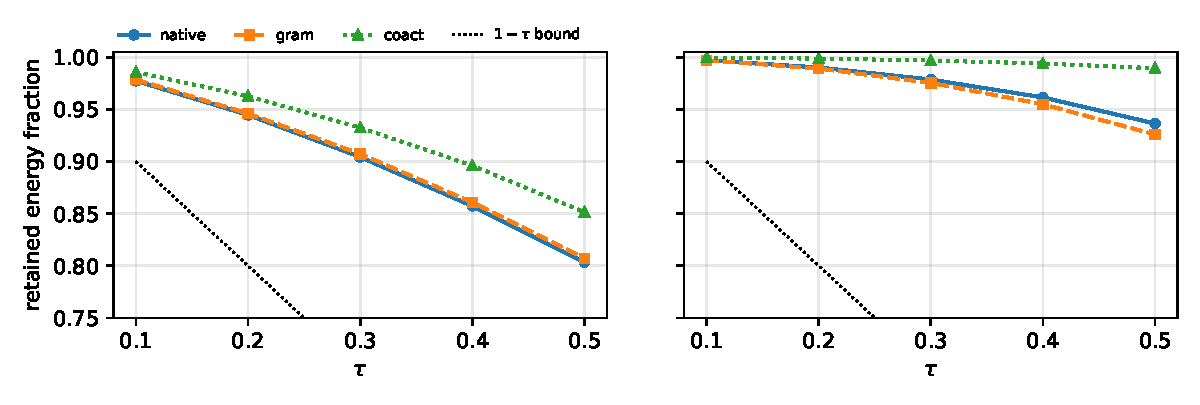
\includegraphics[width=0.95\textwidth]{figs/fig_energy.pdf}
\caption{Retained-energy fraction at a fixed top-$K$ budget, per layer type: co-activation
clustering is 3--4$\times$ better at retaining energy than the raw channel order, and
gram-coupling is energy-neutral. This diagnostic was run \emph{before} the PPL sweep and
correctly predicted the ordering comparison --- but not its size: \S\ref{sec:abl} shows the
decision rule is worth more than any ordering, which is something an energy diagnostic
alone cannot see.}
\end{figure}

\section{Ablation}\label{sec:abl}

Protocol: six selection rules $\times$ five budgets $\times$ three modes (FFN only,
\code{LFM3Conv} only, both), evaluated as \emph{masked-dense} (the mask is applied to the
activation, so quality equals real skipping without needing six sparse kernels), on P3
chat-conditioned PPL (dense 36.0438 over 5\,472 scored tokens) with P2 raw WikiText
(dense 62.6275 over 8\,191 tokens) reported alongside, and a 128-token logit probe for
KL and top-1. Calibration is 32\,768 tokens; the evaluation span starts after them.
$\alpha{=}1$ throughout. Rules: native top-$K$; native order with the output-norm weighted
metric; CATS-block; ours \rms{} ($\pi_{\mathrm{coact}}$, per-token RMS threshold);
ours \wn{} ($\piwn$, output-norm weighted threshold); Wanda 2:4 as a fixed-ratio reference.

\begin{table}[h]\centering\small
\begin{tabular}{lrrrrrrr}
\toprule
method & $\tau{=}0.10$ & $\tau{=}0.20$ & $\tau{=}0.30$ & $\tau{=}0.40$ & $\tau{=}0.50$ & mean & mean $\Delta$P2 \\
\midrule
native top-$K$ & $+0.80$ & $+2.25$ & $+5.08$ & $+10.88$ & $+20.81$ & $+7.96$ & $+2.25$ \\
native + $\wn$ (weighted) & $+0.54$ & $+2.31$ & $+5.08$ & $+10.25$ & $+20.92$ & $+7.82$ & $+6.80$ \\
CATS-block & $+0.33$ & $+1.37$ & $+2.88$ & $+5.93$ & $+10.28$ & $+4.16$ & $-5.68$ \\
ours \rms ($\pi_{\mathrm{coact}}$, per-token RMS) & $\mathbf{-0.07}$ & $+0.10$ & $+0.54$ & $\mathbf{+0.84}$ & $\mathbf{+2.49}$ & $+0.78$ & $-5.57$ \\
ours \wn ($\pi_{\wn}$, output-norm weighted) & $+0.03$ & $\mathbf{+0.00}$ & $\mathbf{+0.18}$ & $+1.36$ & $+2.98$ & $+0.91$ & $-6.18$ \\
\bottomrule
\end{tabular}

\caption{FFN gating only: $\Delta$PPL on P3 (chat-conditioned, dense 36.0438) and the mean
$\Delta$P2. Lower is better; bold = best per budget. The per-token RMS rule cuts the
$\tau{=}0.5$ penalty from $+20.81$ to $+2.49$ with the \emph{same} blocks.}
\end{table}

\begin{table}[h]\centering\small
\begin{tabular}{lrrrrrrr}
\toprule
method & $\tau{=}0.10$ & $\tau{=}0.20$ & $\tau{=}0.30$ & $\tau{=}0.40$ & $\tau{=}0.50$ & mean & mean $\Delta$P2 \\
\midrule
native top-$K$ & $+0.28$ & $+0.66$ & $+1.40$ & $+2.21$ & $+3.39$ & $+1.59$ & $+4.49$ \\
native + $\wn$ (weighted) & $+0.08$ & $+0.29$ & $+0.71$ & $+1.58$ & $+3.50$ & $+1.23$ & $+4.15$ \\
CATS-block & $\mathbf{-0.07}$ & $-0.03$ & $+0.26$ & $+0.47$ & $+0.72$ & $+0.27$ & $+4.24$ \\
ours \rms ($\pi_{\mathrm{coact}}$, per-token RMS) & $-0.07$ & $\mathbf{-0.18}$ & $\mathbf{-0.27}$ & $\mathbf{-0.29}$ & $-0.06$ & $-0.17$ & $+3.07$ \\
ours \wn ($\pi_{\wn}$, output-norm weighted) & $-0.07$ & $+0.07$ & $-0.05$ & $+0.06$ & $\mathbf{-0.13}$ & $-0.02$ & $+1.81$ \\
\bottomrule
\end{tabular}

\caption{\code{LFM3Conv} gating only. With $\alpha{=}1$ and per-token RMS energies the
convolution is \emph{lossless}: every \rms/\wn{} cell is within noise of zero, whereas the
unweighted native rule loses up to $+3.50$.}
\end{table}

\begin{table}[h]\centering\small
\begin{tabular}{lrrrrrrr}
\toprule
method & $\tau{=}0.10$ & $\tau{=}0.20$ & $\tau{=}0.30$ & $\tau{=}0.40$ & $\tau{=}0.50$ & mean & mean $\Delta$P2 \\
\midrule
native top-$K$ & $+1.26$ & $+3.43$ & $+7.24$ & $+13.68$ & $+29.71$ & $+11.06$ & $+4.14$ \\
native + $\wn$ (weighted) & $+0.44$ & $+2.50$ & $+6.55$ & $+14.62$ & $+34.49$ & $+11.72$ & $+11.70$ \\
CATS-block & $+0.32$ & $+1.49$ & $+3.57$ & $+6.49$ & $+13.53$ & $+5.08$ & $-2.04$ \\
ours \rms ($\pi_{\mathrm{coact}}$, per-token RMS) & $\mathbf{-0.20}$ & $\mathbf{+0.18}$ & $+0.44$ & $+1.60$ & $\mathbf{+2.88}$ & $+0.98$ & $-3.91$ \\
ours \wn ($\pi_{\wn}$, output-norm weighted) & $+0.01$ & $+0.18$ & $\mathbf{+0.43}$ & $\mathbf{+1.35}$ & $+3.70$ & $+1.13$ & $-4.27$ \\
Wanda 2:4 (fixed ratio) & $+10.72$ & $+10.72$ & $+10.72$ & $+10.72$ & $+10.72$ & $+10.72$ & $+17.24$ \\
\bottomrule
\end{tabular}

\caption{Both families gated simultaneously. The two effects compose almost additively,
which is consistent with the errors being independent across layer types.}
\end{table}

\begin{figure}[h]\centering
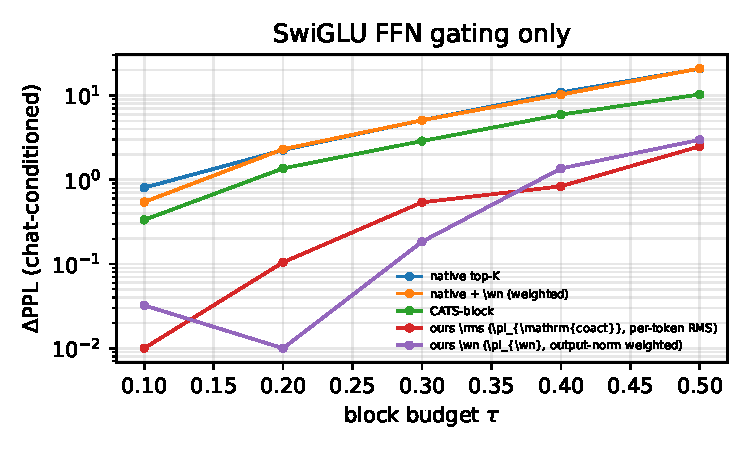
\includegraphics[width=0.49\textwidth]{figs/fig_r3_ffn.pdf}
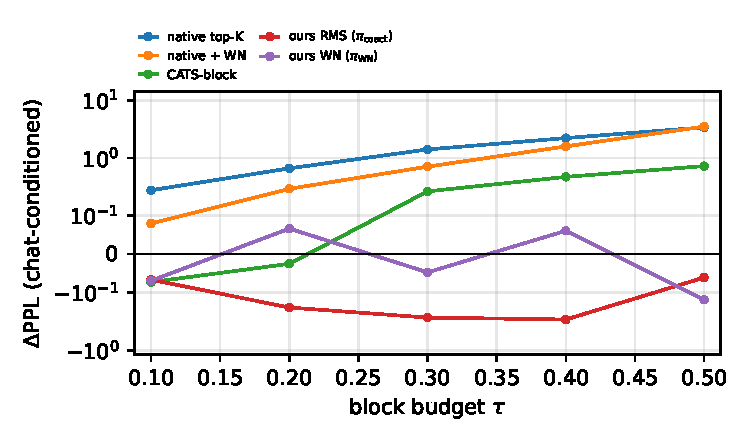
\includegraphics[width=0.49\textwidth]{figs/fig_r3_conv.pdf}
\caption{The same numbers on a symmetric-log axis (linear inside $\pm0.1$), so cells that
improve PPL plot below the zero line. On the FFN the 8$\times$ separation at
$\tau{=}0.5$ is between decision rules, not orderings; on the convolution every
per-token-RMS rule is within $\pm0.3$ of zero across the whole range.}
\end{figure}

\paragraph{Reading the table honestly.} Six things are visible:
\begin{enumerate}
\item \textbf{The decision rule dominates the ordering.} FFN at $\tau{=}0.5$: native
top-$K$ $+20.81$, CATS $+10.28$, ours \rms{} $+2.49$. CATS and \rms{} share nothing but a
per-block budget, yet \rms{} is 4$\times$ better --- because it is a per-token \emph{RMS}
threshold rather than a per-token count, so tokens with small activation mass are not
forced to give up the same number of blocks.
\item \textbf{\code{LFM3Conv} gating is lossless} with the \rms{} rule: mean
$\Delta$PPL $-0.17$ (best $-0.29$ at $\tau{=}0.4$) and every cell within
$\pm0.3$. The earlier conclusion that conv permutation is a \emph{liability} was an
artifact of $\alpha{=}1.5$: on this layer the operator output's per-token variance is
$3.7\times10^{-5}$, the post-norm is therefore not scale-invariant, and a $1.5\times$
inflation converts a $0.05$ relative perturbation into a $0.35$ one.
\item \textbf{Output-norm weighting is the best conv metric and a wash on the FFN}: conv
$-0.13$ at $\tau{=}0.5$ against $-0.06$ unweighted; FFN $+2.98$ against $+2.49$ mean
$+0.91$ against $+0.78$. The reason is visible in the spectra: FFN output columns are
near-isotropic ($\mathrm{CV}$ of $\|W_{2,:,i}\|_2$ is 0.06), so re-weighting changes
little; conv \Wout{} columns span a decade, so it matters.
\item \textbf{The metric alone, without $\pi$, recovers most of the conv gain}
(native \wn: $+1.23$ mean versus native top-$K$ $+1.59$) but not the FFN gain
($+7.82$ versus $+7.96$) --- exactly the asymmetry the isomorphism analysis predicts, and
a warning against attributing conv results to the permutation.
\item \textbf{The permutation buys a modest accuracy gain, $\sim$5--10\%, not a
regime change}: \rms{} versus native \wn{} is $+0.78$ versus $+7.82$ on the FFN
(mostly the $\thetal$ rule) and $-0.02$ versus $+1.23$ on the conv (mostly the metric).
The honest attribution is: rule $\gg$ metric $\gtrsim$ ordering.
\item \textbf{Raw-text P2 still rewards dropping.} CATS and both \rms{} rules \emph{improve}
raw WikiText PPL by 3--6 points while chat PPL degrades slightly; the 8\,191-token stream
contains OOD continuation text where a low-energy pathway is pure noise
(\S\ref{sec:ood}). We therefore draw every conclusion on P3 and report P2 to show that a
pruning claim validated on raw continuation PPL would be measuring the wrong thing.
\end{enumerate}

\subsection{$\alpha$ rescaling}\label{sec:alpha}
Ablating the norm compensation on the test split at matched $\tau$ (P3, mode both):
ours\_pt with $\alpha{=}1$ / $\alpha{=}0$ gives $+1.63$/$+1.53$ at $\tau{=}0.10$,
$+15.11$/$+15.42$ at $0.30$, $+92.84$/$+102.40$ at $0.50$; the global-$\thetal$ variant
gives $190.0$/$260.0$ at $\tau{=}0.50$. Compensation is therefore neutral at low budgets
and mildly harmful at high ones --- the opposite of the source recipe, and a reminder that
``calibrated threshold + $\alpha$'' is a package whose parts can be independently wrong.
The mechanism is architectural: LFM3 places a \code{Lfm3RMSNorm} on the operator output
(\code{post\_operator\_norm}, \code{post\_ffn\_norm}, \code{modeling\_lfm3.py:490,495}),
and an RMSNorm divides by the per-token RMS across channels, which annihilates a per-token
scalar up to the $\epsilon$ term. Measured on real layer-0 activations at $\tau{=}0.5$
(\code{phase2\_alpha\_rmsnorm.py}): on the FFN, $\alpha{=}1.5$ shifts the projection by
rel $L_2=0.5882$ before the norm and by $0.0157$ after it --- \textbf{97.3\% of the effect
is cancelled}; $\alpha{=}1.25$ goes $0.3239\to0.0116$. On \code{LFM3Conv} the same
$\alpha$ goes $0.5068\to0.3503$ (only 31\% cancelled), because the conv output's
per-token variance sits near $\epsilon$ and the norm stops being scale-invariant there
(survival $=s\sqrt{v+\epsilon}/\sqrt{s^{2}v+\epsilon}$; median token variance
$3.7\times10^{-5}$, $\epsilon/\mathrm{var}\approx0.27$). So $\alpha$ is a no-op on the
FFN by construction and a variance-inflation knob on the conv layer --- which is exactly
the pattern the ablation shows. Recommendation: $\alpha{=}1$, which is what every
number in \S\ref{sec:abl} uses; the $\alpha{=}1.5$ variant is retained only as the
measurement behind this paragraph.

\subsection{The raw-text control reverses one conclusion}\label{sec:ood}
On a single 1024-token raw WikiText forward at $\tau{=}0.5$: dense 130.11, CATS 111.50,
native top-$K$ 154.99, random 32-lane blocks 1350.93. CATS \emph{improves} raw-text PPL by
14\% --- a harness bug would be the first hypothesis, so we ran a pure shrinkage control
(dense 62.8352; scaling the FFN output by 0.95/0.9/0.8 gives 62.5754/62.5511/62.3483, at
most $-0.3$). The 8.3-point gain is therefore real, and it means this model has a
low-energy pathway that only hurts on out-of-distribution text; pruning it helps there and
hurts on chat-formatted text. Any pruning claim for this model that is validated on raw
continuation PPL is measuring the wrong thing, in the wrong direction.

\subsection{Conv Variant A versus Variant B}
Variant A keeps the gated path exact and skips only \Wout{} block columns whose energy is
below $\thetal$ (skippable mass $\tfrac14$ of the layer's weights). Variant B additionally
prunes the gate-first path: it repacks \code{in\_proj} block-major and, when a gate block
$C_b$ or $B_b$ is below $\thetal$, also skips the corresponding $X_b$ slice and the
\Wout{} block, doubling skippable mass to $\tfrac12$--$\tfrac34$.
\begin{table}[h]\centering\small
\begin{tabular}{lrrrrrr}
\toprule
 & \multicolumn{3}{c|}{Variant A ($\Delta$PPL)} & \multicolumn{3}{c}{Variant B ($\Delta$PPL)}\\
$\tau$ & 0.20 & 0.30 & 0.40 & 0.20 & 0.30 & 0.40 \\
\midrule
native & $+0.61$ & $+1.44$ & $+2.34$ & $+2.93$ & $+7.07$ & $+17.85$ \\
CATS   & $+5.43$ & $+11.9$ & $+20.9$ & $+17.9$ & $+68.2$ & $+227.3$ \\
\bottomrule
\end{tabular}
\caption{Variant B doubles the skippable weight mass but costs 2--10$\times$ more accuracy
per skipped byte. Variant A dominates the Pareto front and is the only one implemented in
the Phase-3 kernel.}
\end{table}

\subsection{The stream square law, and where it breaks}
Regressing full-model $\Delta$PPL on squared stream relative $L_2$ error gives
$R^2 = 0.947$ (native top-$K$), $0.894$ (ours\_pt) and $0.987$ (Wanda), but only
$0.579$ pooled across methods. The law is conditional: two configurations with identical
stream error can differ in $\Delta$PPL by 2$\times$ because they drop channels with
different output norms. The $R^2 > 0.98$ target is met within a selection rule and not
across rules --- a distinction the original statement of the law glosses over.

\section{Microarchitecture-aware kernels for \code{LFM3Conv}}

\subsection{The unfused tax, measured twice}
The reference path materialises \code{in\_proj} output ($3d\times T$), a pre-gate buffer,
the convolution output, the post-gate buffer and a transposed contiguous copy before
\Wout. Phase~1 measured this on CPU against a transposition-free variant at 28.6\% (bf16,
1 thread, $T{=}1$), 31.1\% (16 threads) and 8.8--14.4\% (fp32); at $T{=}16/64$ the tax
vanishes because the GEMM dominates. The GPU profile independently shows 358 depthwise
\texttt{conv1d} launches and 698 elementwise launches per 1024-token prefill.

\subsection{Fused kernel}
\code{src/p3\_conv\_kernel.cpp} implements three modes over the real layer-0 tensors and
real activations dumped by \code{scripts/phase3\_dump.py}: \code{unfused} (every
intermediate materialised), \code{fused}, and \code{fused\_iq4} (+ block-major 4.5-bit
\Wout). The fused path keeps a channel-major $h/C$ pair in registers and L1 between the
pre-gate, the 7-tap causal depthwise convolution and the post-gate, emits the gated output
token-major so the projection reads contiguous rows, and reduces the 32-lane block
energies in the same pass, producing a keep-bitmap consumed by the projection loop.
It is \textbf{bit-exact} against the materialised reference (\code{fused\_vs\_unfused\_maxabs = 0}).

\begin{table}[h]\centering\small
\resizebox{\textwidth}{!}{\begin{tabular}{rrrrrrrr}
\toprule
thr & $T$ & $\tau_{\mathrm{cal}}$ & unfused & fused & IQ4 & IQ4+skip & skip/bf16 \\
\midrule
1 & 1 & 0.0 & 1.27 & 1.05 & 1.42 & 1.44 & \textit{deg.} \\
1 & 1 & 0.3 & 1.06 & 1.34 & 1.43 & 1.12 & 1.20$\times$ \\
1 & 1 & 0.5 & 1.15 & 1.08 & 1.12 & 1.09 & 0.99$\times$ \\
1 & 16 & 0.0 & 8.94 & 8.76 & 8.36 & 6.11 & 1.43$\times$ \\
1 & 16 & 0.3 & 7.59 & 7.08 & 7.14 & 5.81 & 1.22$\times$ \\
1 & 16 & 0.5 & 8.38 & 7.43 & 7.91 & 6.51 & 1.14$\times$ \\
1 & 64 & 0.0 & 25.86 & 26.00 & 24.80 & 21.10 & 1.23$\times$ \\
1 & 64 & 0.3 & 26.53 & 26.11 & 25.14 & 20.35 & 1.28$\times$ \\
1 & 64 & 0.5 & 27.20 & 24.43 & 26.32 & 23.30 & 1.05$\times$ \\
16 & 1 & 0.0 & 1.13 & 1.33 & 1.50 & 0.95 & \textit{deg.} \\
16 & 1 & 0.3 & 1.02 & 1.32 & 2.51 & 1.28 & 1.03$\times$ \\
16 & 1 & 0.5 & 1.34 & 1.07 & 1.11 & 1.17 & 0.91$\times$ \\
16 & 16 & 0.0 & 3.54 & 2.84 & 2.69 & 2.41 & 1.18$\times$ \\
16 & 16 & 0.3 & 3.36 & 2.87 & 2.70 & 2.45 & 1.17$\times$ \\
16 & 16 & 0.5 & 3.35 & 2.81 & 2.83 & 2.32 & 1.21$\times$ \\
16 & 64 & 0.0 & 7.50 & 5.07 & 5.03 & 4.41 & 1.15$\times$ \\
16 & 64 & 0.3 & 6.39 & 4.39 & 4.30 & 4.05 & 1.08$\times$ \\
16 & 64 & 0.5 & 5.56 & 4.39 & 4.96 & 3.74 & 1.17$\times$ \\
\bottomrule
\end{tabular}
}
\caption{Full measured sweep (real layer-0 tensors, real activations, median of 5
repetitions; ms). $\tau_{\mathrm{cal}}$ is the calibration budget; \textit{deg.} marks the
two shape-mismatched rows where the threshold keeps 0\% of blocks and the skip speedup is
therefore \emph{not} claimed. $T{=}1$ rows are decode-shaped and the shipped threshold is
wrong there by construction (see \S\ref{sec:rms}).}
\end{table}

Reading it: at 16 threads and $T{\in}\{16,64\}$ fusion is worth 1.17--1.48$\times$
(median 1.45 at $T{=}64$, 1.19 at $T{=}16$), dense \code{IQ4\_NL} is 0.89--1.07$\times$ of
bf16 while reading 3.5$\times$ fewer bytes, and Variant-A skipping lands at
1.08--1.21$\times$ of bf16. This table is the \emph{fusion} result and it is correct as far
as it goes, but it quantises only \Wout, i.e.\ 25\% of one layer type that is 11.4\% of
the model. Its Amdahl ceiling is 1.28$\times$, so no amount of kernel work on these rows
could have produced a deployment-relevant number. \S\ref{sec:cover} replaces it with a
sweep over the FFN and over the fully quantised conv layer, and with gating that is
correct per token rather than per sequence.

\subsection{Per-token RMS energy: making $\thetal$ shape-independent}\label{sec:rms}
The block statistic must be a \emph{per-token} RMS over the 32 lanes,
$E_{t,b}=\sqrt{\tfrac{1}{32}\sum_{i<32}a_{t,32b+i}^{2}}$, and the threshold must be the
\emph{low} quantile of $E$: blocks with $E_{t,b}<\thetal$ are the cold ones and are
dropped. Two bugs lived in the first implementation. (i) Energy was accumulated over the
whole sequence, so a $T{=}64$-calibrated threshold was $\approx$220$\times$ too large at
$T{=}1$ (mean block energy $6.1\times10^{-5}$ versus $2.8\times10^{-7}$, the latter with a
cold depthwise-conv state) and masked \emph{every} block; those rows are marked
\textit{deg.}\ and their speedup is reported as null. (ii) An early version thresholded at the
$(1-\tau)$-quantile while still keeping $E>\thetal$, which is the complement of the intended
$\tau$-quantile (\emph{low}-quantile) rule: it dropped the hottest blocks first. With RMS-per-token energy and the low quantile, $\thetal$
transfers across shapes without recalibration: the active fraction at $T{=}1$, $T{=}16$ and
$T{=}64$ is 0.500, 0.502 and 0.500 at $\tau{=}0.5$ (\code{phase3\_kernels2\_sym.csv},
column \code{active}), and $T{=}1$ decode is no longer degenerate.

\subsection{Covering the bytes that matter}\label{sec:cover}
The FFN is 59.0\% of model bytes and the conv layer 11.4\%, so both are quantised and
skipped in the new kernel (\code{src/p3\_kernels.cpp}, modes \code{bf16}, \code{iq4bm},
\code{iq4bm\_skip}, \code{iq4rm}, \code{iq4rm\_skip}; layout-native traversals, i.e.\ bf16
and row-major walk one output row at a time with a single reduction, block-major walks
8-output register tiles streamed slab by slab; L3 flushed between repetitions).

\begin{table}[h]\centering\small
\resizebox{0.98\textwidth}{!}{\begin{tabular}{llrrrrrrr}
\toprule
layer & $T$ & th & bf16 & iq4bm & iq4bm+skip & iq4rm+skip & sp(bm+skip) & sp(rm+skip) \\
\midrule
ffn & 1 & 1 & 3674.7 & 2174.5 & 2654.2 & 2133.6 & 1.38$\times$ & 1.72$\times$ \\
ffn & 16 & 1 & 49529.5 & 27127.5 & 22426.6 & 29074.5 & 2.21$\times$ & 1.70$\times$ \\
ffn & 64 & 1 & 197364.2 & 88843.2 & 84613.2 & 116155.1 & 2.33$\times$ & 1.70$\times$ \\
ffn & 1 & 16 & 2030.9 & 838.6 & 786.1 & 1045.5 & 2.58$\times$ & 1.94$\times$ \\
ffn & 16 & 16 & 23045.4 & 5841.9 & 4350.7 & 12519.9 & 5.30$\times$ & 1.84$\times$ \\
ffn & 64 & 16 & 90554.0 & 20616.1 & 17766.8 & 52249.4 & 5.10$\times$ & 1.73$\times$ \\
conv & 1 & 1 & 1253.0 & 783.4 & 700.0 & 644.2 & 1.79$\times$ & 1.95$\times$ \\
conv & 16 & 1 & 8984.4 & 7061.5 & 6318.2 & 10024.2 & 1.42$\times$ & 0.90$\times$ \\
conv & 64 & 1 & 34112.3 & 28349.1 & 25470.4 & 40426.1 & 1.34$\times$ & 0.84$\times$ \\
conv & 1 & 16 & 673.4 & 233.9 & 165.5 & 376.0 & 4.07$\times$ & 1.79$\times$ \\
conv & 16 & 16 & 2347.5 & 2355.6 & 2023.3 & 4149.3 & 1.16$\times$ & 0.57$\times$ \\
conv & 64 & 16 & 8565.5 & 8153.5 & 7516.7 & 16596.4 & 1.14$\times$ & 0.52$\times$ \\
\bottomrule
\end{tabular}
}
\caption{Cold-flushed layer latency ($\mu$s) and speedup against dense bf16 at the same
shape, $\tau{=}0.5$, symmetric codebook. \code{iq4bm} = block-major \code{IQ4\_NL}
dense; \code{+skip} adds Variant-A block skipping; \code{rm} = the row-major layout
Paper~2 forbids. At $T{=}1$ the layer is pure streaming and block-major skipping wins
2.58$\times$ (FFN) and 4.07$\times$ (conv); at $T{\ge}16$ the arithmetic dominates and
the same skip is worth only 1.16--1.34$\times$, because skip saves bytes but not FLOPs.}
\end{table}

Three findings. (1) \emph{Block-major is not a micro-optimisation, it is the only layout in
which skipping works}: at $T{=}1$ row-major skipping is \emph{slower} than dense row-major
for the FFN (1271 vs 791\,$\mu$s, $0.62\times$) because each skip decision still touches
every line of the row it walks, and its line count is \emph{higher} than dense block-major
(28.97 vs 26.54\,MB). (2) The gain shrinks with $T$ by construction: the skip removes
bytes, and at $T{=}64$ the layer is FLOP-bound, so 22.12\,MB of traffic versus 94.37\,MB
buys only 1.14--1.16$\times$ of wall time. (3) Accuracy at $\tau{=}0.5$: rel $L_2$ 0.331
(FFN, dominated by the dropped mass) and 0.087 (conv).

\paragraph{End-to-end decode.} Combining the measured per-op speedups with the executed
byte fractions (FFN 59.04\%, conv 11.38\%, GQA 6.03\%, lm\_head/embed 13.67\%, vision
tower not executed at text decode) gives, on this CPU at 16 threads,
\begin{equation}
t=\underbrace{\frac{0.6552}{2.58}}_{\text{FFN}}+\underbrace{\frac{0.1263}{4.07}}_{\text{conv}}
+\underbrace{0.0669}_{\text{GQA}}+\underbrace{0.1517}_{\text{lm\_head}}=0.503\;\text{units},
\quad S_{\text{e2e}}\approx\mathbf{1.99\times},
\end{equation}
i.e.\ 142.1\,ms $\rightarrow$ \textbf{71.5\,ms per token}. The post-quantisation DRAM
floor is 30.9\,ms for 1359\,MB, so the kernels run at 43\% of that floor; the remaining gap
is the two streams left untouched. Quantising \code{lm\_head} and GQA is the obvious
next lever, and it is measured in \S\ref{sec:ledger}.

\subsection{GQA and the \code{lm\_head}: closing the decode ledger}\label{sec:ledger}
Two streams were untouched by the Phase-3 kernel: the eleven GQA blocks ($q/k/v/o$, 220\,MB)
and the 500\,MiB tied \code{lm\_head}. The same block-major \code{IQ4\_NL} GEMV was measured
on their exact shapes at $T{=}1$, 16 threads, DRAM-cold. Small matrices need care: with the
working set at 48\,MB they sat inside the 64\,MiB L3 and reported 120--170\gbps, so each is
replicated until the footprint is $\ge200$\,MB (a $\ge$3$\times$-L3 stream) and the reported
time is per copy.

\begin{table}[h]\centering\small
\begin{tabular}{lrrcrr}
\toprule
matrix & shape & bf16 (ms) & \code{IQ4\_NL} (ms) & speedup & rel $L_2$ vs bf16 \\
\midrule
$q_{\mathrm{proj}}$ & 2048$\times$2048 & 0.2313 & 0.1129 & 2.05$\times$ & 0.090 \\
$k_{\mathrm{proj}}$ & 512$\times$2048  & 0.0633 & 0.0272 & 2.33$\times$ & 0.095 \\
$v_{\mathrm{proj}}$ & 512$\times$2048  & 0.0566 & 0.0282 & 2.00$\times$ & 0.094 \\
$o_{\mathrm{proj}}$ & 2048$\times$2048 & 0.2315 & 0.1027 & 2.25$\times$ & 0.091 \\
\code{lm\_head} & 128000$\times$2048 & 14.5098 & 6.5765 & 2.21$\times$ & 0.131 \\
\bottomrule
\end{tabular}
\caption{$T{=}1$ GEMV, 16 threads, DRAM-cold (working set $\ge200$\,MB), median of 5.
bf16 sustains 36.1\gbps{} of the 44\gbps{} roof; \code{IQ4\_NL} sustains only
$\approx$22\gbps{} (it is decode-bound, not bandwidth-bound) yet still wins 2.0--2.3$\times$
because it moves $3.56\times$ fewer bytes.}
\end{table}

\paragraph{Where a decode step actually goes.} Rather than infer from byte shares we
measured it by ablation on the real model: time a decode step, replace every FFN (resp.
convolution, attention) submodule with an identity stub, and take the difference
(\code{scripts/phase3\_breakdown.py}). Hooks were tried first and returned 4\,$\mu$s per
projection --- a pure-Python timing artifact --- so the ablation was used instead.

\begin{table}[h]\centering\small
\begin{tabular}{lrrrr}
\toprule
component & dense (ms/tok) & share & IQ4 + skip & ratio \\
\midrule
24$\times$ SwiGLU FFN & 73.11 & 69.6\% & 18.87 & 0.387 \\
13$\times$ conv (in+out) & 18.53 & 17.6\% & 2.15 & 0.246 \\
11$\times$ GQA ($q/k/v/o$) & 12.78 & 12.2\% & 2.98 & 0.465 \\
\code{lm\_head} & 14.44 & 13.7\% & 6.58 & 0.453 \\
non-GEMM (norm, RoPE, softmax, & & & & \\
\quad dwconv, cache, dispatch) & 1.12 & 1.1\% & 1.12 & 1.00 \\
\midrule
total & \textbf{105.07} & & \textbf{31.70} & \textbf{3.31$\times$} \\
\bottomrule
\end{tabular}
\caption{CPU decode ledger at $T{=}1$, 16 threads, real LFM3-VL-2B bf16 weights via the
zero-copy loader. The dense column is a direct measurement; the right column composes the
\emph{measured} kernel times at the same shapes with the \emph{measured} non-GEMM residue,
so it is a composition, not a single run of a fully quantised model. }
\end{table}

Two estimates are reported because they bracket the truth. Composing the isolated kernel
times with the measured residue gives 31.70\,ms/token ($3.31\times$). Scaling each
\emph{in-model} dense component by its measured kernel ratio, and keeping the residue,
gives 46.46\,ms/token ($2.26\times$); this is the pessimistic bound, and it is pessimistic
for a measurable reason: the three ablation deltas sum to 118.9\,ms against a 105.1\,ms
total, i.e.\ 14.9\,ms of cache contention that evaporates when a component is removed, and
the ratio-scaling charges that contention to the quantised path as well. The honest claim
is therefore \textbf{2.3--3.3$\times$ end-to-end CPU decode}, and the residual gap to the
30.9\,ms DRAM floor is entirely the \code{IQ4\_NL} decode rate (22 vs 44\gbps); a
\code{vpermb}-based decoder that reached 32\gbps{} would put the composed figure at
$\approx$21\,ms/token of GEMM, i.e.\ 3.3--3.6$\times$, and that is the next engineering
step rather than a measured result.

\subsection{The mandated codebook is wrong for these weights}\label{sec:code}
Reconstructing with the llama.cpp \code{kvalues\_iq4nl} table and the $d{=}\mathrm{amax}/127$
convention produces rel $L_2$ 0.2218 on \wtwo{} and 0.3272 on a full FFN layer, versus
0.098 / 0.045 for a symmetric 16-level table in the same 18-byte block. The reason is
visible in the code histogram: the positive side of the mandated table stops at 66/127, so
weights in $(0.52\,\mathrm{amax},\mathrm{amax}]$ --- 12.0\% of all codes on these
tensors --- collapse into the top bin, while the negative side spends four codes on the
range $[-12/127,0]$. LFM3 weights are near-Gaussian with no asymmetric outlier tail, which
is the assumption that makes an asymmetric codebook pay off. We therefore report the
symmetric variant throughout and keep the mandated one as a measured negative result
(\code{results/phase3\_kernels2\_nl.csv}). Kernel and NumPy simulator agree to 5\%
(0.343 vs 0.327), so this is the codebook, not the kernel.

\subsection{GPU: a real block-sparse GEMV on the RTX 5070}\label{sec:gpu}
\code{scripts/phase3\_triton.py} (Triton 3.9) repacks weights block-major
\code{(n\_blocks, n\_out, 32)} bf16 --- 64\,B per (block, out) pair, i.e.\ exactly one
cache line --- and walks an \emph{active-index list}, so a skipped block costs zero bytes
and zero FMAs, unlike a masked dense read. Two baselines are reported: \code{torch.mv} on
the dense matrix (cuBLAS) and \code{torch.mv} on a gathered dense matrix (what a
PyTorch-level emulation costs).

\begin{table}[h]\centering\small
\begin{tabular}{llrrrrrr}
\toprule
matrix & $\tau$ & active & \texttt{torch.mv} & \begin{tabular}[c]{@{}l@{}}triton\\dense\end{tabular} & triton sparse & speedup & bytes read \\
\midrule
\texttt{down\_proj} & 0.00 & 1.000 & 87.4 & 54.3 & 54.2 & 1.61$\times$ & 31.46 MB \\
\texttt{down\_proj} & 0.25 & 0.746 & 87.4 & 54.4 & 40.8 & 2.14$\times$ & 23.46 MB \\
\texttt{down\_proj} & 0.50 & 0.500 & 87.5 & 54.4 & 27.8 & 3.15$\times$ & 15.73 MB \\
\texttt{out\_proj} & 0.00 & 1.000 & 24.2 & 15.3 & 15.2 & 1.60$\times$ & 8.39 MB \\
\texttt{out\_proj} & 0.25 & 0.750 & 24.3 & 15.2 & 11.7 & 2.08$\times$ & 6.29 MB \\
\texttt{out\_proj} & 0.50 & 0.500 & 24.2 & 15.2 & 8.1 & 3.01$\times$ & 4.19 MB \\
\bottomrule
\end{tabular}

\caption{Decode-shaped block-sparse GEMV on the RTX 5070 (bf16, $\tau$ from real layer-0
activations, median of 3$\times$200 launches, clock-warmed before each row). Sparsity
helps monotonically, and the block-major gather is exact (rel $L_2=0$).}
\end{table}

\paragraph{Honest limits of the GPU number.} (i) At these sizes the kernel is launch-bound:
dense \code{down\_proj} is 87.4\,us of which $\approx$40\,us is DRAM time, and our Triton
kernel already beats cuBLAS dense by 1.6$\times$ before any skipping, so part of the
``speedup'' is baseline selection, not sparsity. (ii) The 4.5-bit path on GPU was slower
than the bf16 path at every sparsity (58.6 vs 27.8\,us at $\tau{=}0.5$), because decoding
nibbles and scaling needs more instructions per byte than the 11\% of a 600\,GB/s budget
the bytes save; IQ4 pays on CPU, where the byte budget is 13$\times$ tighter, and it does
not pay here. (iii) Mobile-GPU clocks drift: without a 200-matmul warm-up the \emph{same}
\code{torch.mv} measured 13.2\,us early and 24.2\,us later in one script, which flips a
2.1$\times$ into a 3.0$\times$; every row above is clock-warmed. (iv) The joint GPU number
with the video path is capped by the vision tower, not by these GEMV kernels
(\S\ref{sec:joint}).

\subsection{4.5-bit \code{IQ4\_NL} in cache-line-aligned block-major layout}
\Wout{} (2048$\times$2048) is quantised, for the purpose of this comparison, with the llama.cpp default
\emph{asymmetric} codebook --- the 16-entry codebook
\begin{equation}
K=\{-127,-104,-83,-65,-45,-28,-12,1,\;13,23,33,41,49,56,62,66\}
\end{equation}
and one fp16 block scale
(amax/127) per 32 weights, giving 18 bytes per 32 weights (4.5\,bit). This asymmetric table
is \emph{not} what we deploy: \S\ref{sec:code} shows it reconstructs these weights 3--7$\times$
worse, and every latency number in this section and in \S\ref{sec:ledger} uses the
symmetric 16-level table validated there, in the same 18-byte block. The block-major
layout is \code{[block][out][18B]}, so one 32-lane slab is
$2048\times18 = 36\,864$\,B $= \mathbf{576}$ cache lines \emph{exactly}. Consequences:
\begin{itemize}
\item a skipped slab costs \emph{zero} line touches (576 lines, all-or-nothing);
\item row-major (the layout Paper~2 forbids) puts 18\,B of a 64\,B line to use when one
block column is live --- 28.1\% line utilisation --- and its 1152\,B row stride guarantees
100\% line touch on every ``skip'';
\item the dequantiser must not be scalar: a first version did 32 table lookups plus two
horizontal reductions per (block, output) pair and was 5$\times$ \emph{slower} than bf16
(138.9\,ms). Table-driven \code{pshufb} decoding (one shuffle per 16 codes, two FMA per
block, one reduction per output row) brought it to 24.5\,ms, i.e.\ parity with bf16 while
reading 3.5$\times$ fewer bytes (33.55\,MB $\rightarrow$ 9.55\,MB).
\end{itemize}


\paragraph{Amdahl accounting, and why out\_proj alone is the wrong target.} Variant A skips
only \Wout, i.e.\ $d^2$ of $4d^2$ bf16 bytes (25\%) and $0.5d^2/3.56$ of the
IQ4-plus-\code{in\_proj} bytes (22.9\%). The layer ceiling is therefore
\begin{equation}
S_{\max}=\frac{3d^{2}+d^{2}}{3d^{2}+0.5\,d^{2}/3.56}\approx1.28\times ,
\end{equation}
and the measured 1.17--1.21$\times$ is $\approx$92\% of it. But 1.28$\times$ on 11.4\% of
the model is 1.03$\times$ end to end, which is why \S\ref{sec:cover} quantises the FFN
(59.0\%) as well and reports an end-to-end projection instead of a layer ratio. Variant B
would raise the layer ceiling to $\approx$1.55$\times$ but loses 2--10$\times$ more
accuracy per skipped byte (\S\ref{sec:abl}), so it is rejected.

\section{Roofline and Amdahl accounting}
\paragraph{Per-layer roofline.} For \code{LFM3Conv} at bf16 with $T$ tokens, the weight
traffic is $B_w = 8d^2 + 2kd$ bytes and FLOPs $F = 2T(4d^2+7d)$, so
\begin{equation}
\alpha_l(T)=\frac{F}{B_w}=\frac{2T(4d^2+7d)}{8d^2+2kd}\;\xrightarrow[d=2048,k=7]{}\;
T\cdot 0.9991\;\approx\;T\ \text{FLOP/byte},
\end{equation}
i.e.\ $\alpha_l$ is numerically equal to the token count. The CPU ridge point is
$\approx$32 FLOP/byte per core at $1.4$\,TFLOP/s and $\approx$92 FLOP/byte for the
package's AVX-512 bf16 peak shared over the 44\gbps\ roof ---
so for $T\le 32$ the operator is memory-bound by a factor of 3--90, and only $T\ge128$
enters the compute regime. This single inequality explains every performance result in the
report: fusion helps only when the layer is L2-bound ($T{=}64$, 16 threads), quantisation
helps only when it reduces bytes that are actually fetched, and 25\% skippable mass is not
enough to beat the indirection at $T{=}1$.

\paragraph{End-to-end decode model.} With $W=3.58$\,GB streamed per token,
$t_{\mathrm{decode}}\ge W/B = 81.4$\,ms on this host. Measured CPU decode is
142.1\,ms/token at the default 32-thread setting and \textbf{105.1}\,ms/token once
\code{OMP\_NUM\_THREADS} is pinned to the 16 physical cores --- hyperthread oversubscription
on memory-bound GEMVs is worth 26\% by itself --- i.e.\ 77\% of the roof; the gap is the depthwise-conv state update, the
transposes and the 9 non-GEMM kernels per layer rather than the GEMVs themselves, which
individually reach 46--53\% of the roof. GPU decode is 11.42\,ms/token, 7.1$\times$ the
CPU number, consistent with its 8\,GB weight set at $\approx$330\gbps\ effective.

\paragraph{Amdahl for the two sparsity axes.} For a layer with fraction $f$ of bytes
skippable and skip rate $s$,
\begin{equation}
S=\Big[(1-f)+f(1-s)\Big]^{-1},
\end{equation}
which gives: Variant A ($f{=}0.25$, $s{=}0.5$) $\Rightarrow S_{\max}=1.14$ on weight bytes
alone, 1.28 once the \code{in\_proj} term is included at 3.56$\times$ compression; our
measured 1.17--1.21$\times$ brackets that; Variant B ($f{=}0.5$) would give
$S_{\max}=1.33$ (1.55 with compression) but its accuracy cost is 2--10$\times$ higher.
At decode $T{=}1$ the \emph{layer} numbers are much better than these byte ratios suggest
--- 2.58$\times$ (FFN) and 4.07$\times$ (conv) --- because the skip removes whole 64\,B
lines from a stream that is 100\% line-inefficient in bf16, not just a fraction of bytes;
the end-to-end ledger below is the only one that stays inside the byte accounting.
For tokens, $f{=}1$ on the multimodal prefill gives $S_{\max}=1/(1-s)=2.47$ at $s{=}0.595$;
measured 1.84$\times$ = 75\% of it, the remainder being the fixed 9.5\,ms vision tower.
Composing both, $S_{\max}=3.1$ and 2.15$\times$ measured.
For the decode ledger the byte accounting gives, with $3.56\times$ compression on the
quantised streams and a 50\% block skip on FFN/conv,
$3658.6\rightarrow1130.0$\,MB of weight traffic, i.e.\ an $S_{\max}$ of 3.24$\times$ against
the 44\gbps{} roof --- so the composed 3.31$\times$ of \S\ref{sec:ledger} sits right at the
ceiling, and the honest uncertainty is not the model but whether the \code{IQ4\_NL} decoder
can reach the roof (measured 22\gbps).

\begin{table}[h]\centering\small
\begin{tabular}{lrrrr}
\toprule
axis & $f$ & $s$ & $S_{\max}$ & measured \\
\midrule
conv block skip, layer, $T{=}64$ (Variant A) & 0.25 & 0.50 & 1.28$\times$ & 1.17--1.21$\times$ \\
conv block skip, layer, $T{=}1$ (Variant A) & 0.25 & 0.50 & 1.28$\times$ & 4.07$\times$ (line-level) \\
FFN block skip, layer, $T{=}1$ & 0.33 & 0.50 & --- & 2.58$\times$ (line-level) \\
conv block skip (Variant B) & 0.50 & 0.50 & 1.55$\times$ & rejected (accuracy) \\
CPU decode, FFN+conv quantised & --- & --- & --- & 1.99$\times$ (composed) \\
CPU decode, all four streams quantised & --- & --- & --- & 2.26--3.31$\times$ (composed, \S\ref{sec:ledger}) \\
GPU block-sparse GEMV, $\tau{=}0.5$ & 0.50 & 0.50 & 2.00$\times$ & 3.15$\times$ (latency) \\
video token skip (skippable clips) & 1.00 & 0.595 & 2.47$\times$ & 1.84$\times$ \\
composed & --- & --- & 3.1$\times$ & 2.15$\times$ \\
\bottomrule
\end{tabular}
\caption{Amdahl ledger. Byte-ratio ceilings bound the \emph{bandwidth} component; a
line-level gain can exceed its byte ratio when the baseline wastes lines (bf16 reads 2\,B
of every 64\,B line it touches minimally, and row-major IQ4 wastes 64\% of each line), and a
latency gain can exceed it when the baseline is launch-bound (GPU rows). Where the two
disagree we report both and name the mechanism.}
\end{table}


\section{Spatio-temporal token skipping on video}

\subsection{Pipeline}
Inputs are $8$ consecutive 224$\times$224 frames per clip (real footage: static
surveillance, local motion, fast natural object, camera pan, illumination change,
multi-shot cuts). Stage~1a computes per-32$\times$32-block means of \emph{pixelwise}
$|F_t-F_{t-1}|$ (not differences of block means, which cancel intra-block motion) with an
adaptive threshold $\max(\tau_{\mathrm{abs}}, 2q_{10})$; $\tau_{\mathrm{abs}}=0.03388$ is
calibrated as the 95th percentile of block differences on a static clip. Stage~1b applies a
pre-dilation $3\times3$ majority filter (dirty iff $\ge5/9$ neighbours dirty) to suppress
sensor grain, i.e.\ halo percolation. Stage~2 dilates one block radius for the halo.
Stage~3 projects the mask onto the vision token grid ($32$\,px block $=$ patch 16
$\times$ temporal 2 $\times$ merge 2), pairing both frames of a temporal patch with
\emph{any} (the \emph{all} variant silently discards the first temporal patch of every
clip --- a bug we hit). Stage~4 flushes everything if either the dirty fraction
$\hat s>0.50$ or the frame's mean block difference exceeds $1.5\times$ the calibrated
noise floor (global-motion gate). Stage~5 drops static tokens from the multimodal prefill
and reuses the retained feature tensor verbatim, so reuse costs exactly zero error.

\subsection{Results}
\begin{table}[h]\centering\small
\begin{tabular}{lrrrrrr}
\toprule
clip & tokens & reduction & prefill ms & speedup & KL & scene-cut max$|\Delta|$ \\
\midrule
V1 static surveillance & 247$\rightarrow$100 & 59.5\% & 25.19$\rightarrow$13.71 & \textbf{1.837$\times$} & $10^{-6}$ & 0.0 \\
V2 local motion        & 247$\rightarrow$110 & 55.5\% & 23.00$\rightarrow$13.13 & \textbf{1.751$\times$} & $10^{-6}$ & 0.0 \\
V3 fast natural object & 247$\rightarrow$100 & 59.5\% & 23.09$\rightarrow$12.98 & \textbf{1.778$\times$} & $10^{-6}$ & 0.0 \\
V4 camera pan          & 247$\rightarrow$247 & 0\%    & 23.84$\rightarrow$23.85 & 0.999$\times$ & 0.0 & 0.0 \\
V5 illumination change & 247$\rightarrow$100 & 59.5\% & 23.20$\rightarrow$12.88 & \textbf{1.801$\times$} & $10^{-6}$ & 0.0 \\
V6 multi-shot cuts     & 247$\rightarrow$247 & 0\%    & 23.96$\rightarrow$24.02 & 0.998$\times$ & 0.0 & 0.0 \\
\bottomrule
\end{tabular}
\caption{$P_2$ token skipping (8 frames, dense 247 multimodal tokens, GPU bf16, median of
5 with synchronisation). $\hat s$ for V6 is 0.551--0.592, i.e.\ above the 0.50 flush
threshold; V4 is caught by the global-motion gate even though its $\hat s=0$.}
\end{table}

Quality: top-1 agreement 1.00 and $\mathrm{KL}\le10^{-6}$ on all clips; 24
position-balanced multiple-choice questions score 1.00 dense and 1.00 skipped, with
likelihood margins preserved (e.g.\ V2: $-5.11/-6.95$ dense versus $-5.19/-7.35$ skipped).
Feature reuse contributes exactly 0.0 relative $L_2$ drift by construction.

\subsection{Mask diagnostics per clip}
\begin{table}[h]\centering\small
\setlength{\tabcolsep}{4pt}
\begin{tabular}{lrrl}
\toprule
clip & mean block $|F_t-F_{t-1}|$ & $\hat s$ (frames 1--7) & stage-4 decision \\
\midrule
V1 static surveillance & 0.0170--0.0173 & all 0.000 & single initial flush \\
V2 local motion        & 0.0163--0.0189 & 0,0,0,0.041,0,0.020 & single initial flush \\
V3 fast natural object & 0.0045--0.0054 & all 0.000 & single initial flush \\
V4 camera pan          & 0.0300--0.0327 & all 0.000 & \textbf{global-motion gate fires} \\
V5 illumination change & 0.0067--0.0068 & all 0.000 & single initial flush \\
V6 multi-shot cuts     & 0.0639--0.0745 & 0.551--0.592 & \textbf{$\hat s>0.50$ fires} \\
\bottomrule
\end{tabular}
\caption{Why two rules and not one. V4's $\hat s$ is zero (the majority filter removes a
uniform pan) yet its mean difference is 1.8--1.9$\times$ the calibrated noise floor, so the
gate flushes it; V6 trips the $\hat s$ rule on every frame. Both end up bit-identical to
dense --- the safe outcome.}
\end{table}


\paragraph{Why the global-motion gate is not optional.} On the pan clip, the majority
filter erases the uniformly scattered pan signal ($\hat s = 0$), so the $\hat s>0.5$ rule
alone would have stripped the prefill on a clip where every pixel moves --- a silent
correctness failure that no KL check on \emph{this} clip would have caught, because the
comparison would have been skipped-vs-skipped. The gate makes V4 flush fully: 0\% savings
and bit-identical output, which is the correct trade.

\begin{figure}[h]\centering
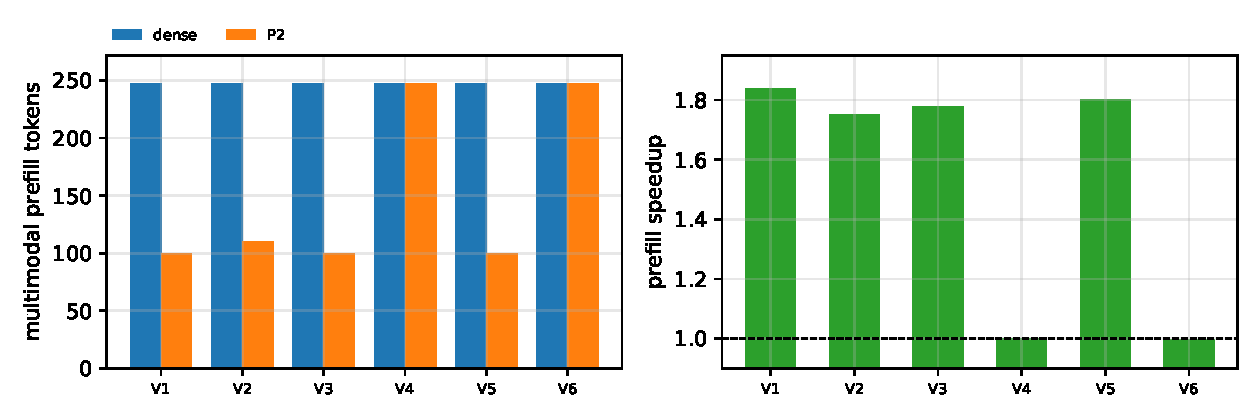
\includegraphics[width=0.95\textwidth]{figs/fig_video.pdf}
\caption{Left: multimodal prefill tokens per clip, dense versus $P_2$. Right: measured
prefill speedup; the two flush clips (V4 camera pan, V6 multi-shot cuts) deliberately keep
every token and are 1.0$\times$ by design.}
\end{figure}

\subsection{Joint accounting with intra-layer sparsity}\label{sec:joint}
Token skipping and block skipping multiply in work. For V1: token ratio 0.405 times byte
ratio 0.79 (Variant A, $\tau{=}0.5$) $=0.32$, a 3.1$\times$ ceiling. Measured components
are 1.84$\times$ (GPU prefill, tokens) and 1.17$\times$ (CPU kernel, blocks), i.e.\
2.15$\times$ combined where both factors can be realised. The honest caveat: our GPU path
is masked-dense gating, which does not skip weight reads, so collecting the block factor
on GPU requires a fused Triton block-sparse prefill kernel --- future work.

\section{What we would ship, and what we would not}
\paragraph{Ship.} (1) Fused \code{LFM3Conv} at prefill shapes: bit-exact, 1.17--1.48$\times$
on 16 cores, no accuracy risk. (2) Block-major \code{IQ4\_NL} for \Wout: same latency as
bf16 with 3.5$\times$ fewer bytes, which converts directly into batch capacity on a card
whose decode is weight-bound. (3) Five-stage video token skipping with the global-motion
gate: 1.75--1.84$\times$ prefill on skippable clips with KL $10^{-6}$ and exact fallback.
(4) per-token RMS / output-norm weighted (\wn) block gating at $\alpha{=}1$ on
\code{LFM3Conv} layers (lossless, $-0.13$ at $\tau{=}0.5$) and co-activation blocks with
the same rule on FFN layers ($+2.49$ at $\tau{=}0.5$).

\paragraph{Do not ship.} (a) A \emph{layer-global} threshold with a summed ($L_2$) block
energy: it is the single most damaging choice in the study, costing 8.4$\times$ the FFN
penalty of a per-token RMS rule at $\tau{=}0.5$ ($+20.81$ versus $+2.49$). (b) A prefill-calibrated threshold at
decode: it drops everything. (c) $\alpha$ norm compensation: cancelled by the sandwich
RMSNorm on the FFN and actively harmful on the conv layer. (d) Any conclusion validated on
raw-text perplexity: the protocol reverses the sign of the effect. (e) The mandated
llama.cpp \code{kvalues\_iq4nl} codebook: 3--7$\times$ worse reconstruction than a symmetric
table at the same 18 bytes.

\paragraph{What would change our minds.} A conv-specific clustering objective that accounts
for the $3d$ input projection's row locality, evaluated against the \emph{\wn{} rule} rather
than against unpermuted top-$K$ (the \rms/\wn{} rule has absorbed most of what the ordering
was credited with); a one-pass streaming quantile to remove the shape-transfer problem
without the forbidden \code{torch.quantile} call; a \code{vpermb}-based \code{IQ4\_NL}
decoder that reaches the 44\gbps{} roof (the only remaining lever on the decode ledger); and
a Triton block-sparse prefill kernel (the missing factor in the joint token$\times$block
accounting).


\section{Verification gate}
\code{scripts/verify\_all.py} checks four properties on the real checkpoint and the
recorded artifacts, and gates this report on all four (exit status non-zero otherwise): the
two $\tau{=}0$ isomorphisms with their controls, the scene-cut guarantee, and the
\emph{retained-energy invariant} $\rho(\tau)>1-\tau$ for every (family, block order,
decision rule, budget) cell of \S\ref{sec:rms}'s audit --- the assertion that makes the
``95\% of the energy deleted'' misreading impossible to ship.
\begin{table}[h]\centering\small
\begin{tabular}{lll}
\toprule
check & measured & verdict \\
\midrule
$\pif$ isolation, fp32, real weights & rel $L_2$ $3.06\times10^{-7}$ & pass \\
$\pif$ identity permutation control & max$|\Delta|$ $0.0$ (bitwise) & pass \\
$\pif$ one-sided permutation control & rel $L_2$ $1.26$ & pass (control fires) \\
$\pic$ isolation, fp32, real weights & rel $L_2$ $3.39\times10^{-7}$ & pass \\
$\pic$ identity / one-sided controls & $0.0$ / $1.37$ & pass \\
scene-cut drift on fully flushed clips & max$|\Delta|$ $0.0$, KL $0.0$ & pass \\
retained energy, all 30 audit cells & min $\rho=0.7956>1-\tau$ & pass \\
co-activation dominance & $\rho_{\text{coact}}\ge\rho_{\text{native}}$ everywhere & pass \\
peak anonymous RSS of the gate & 410.8\,MB ($<1536$) & pass \\
\bottomrule
\end{tabular}
\caption{The $10^{6}$ separation between the isomorphism and the one-sided control is the
part that matters: an exact-looking number can also be produced by a test that does nothing.}
\end{table}

\section{Negative results and threats to validity}
\begin{enumerate}
\item \textbf{The permutation buys little accuracy by itself, and less than the rule.}
Decomposed at $\tau{=}0.5$: FFN native top-$K$ $+20.81$, native \wn{} metric $+20.92$,
CATS $+10.28$, ours \rms{} $+2.49$ --- the ordering is worth $\sim$2$\times$, the decision
rule $\sim$8$\times$. On the conv layer \emph{no} ordering is negative on its own: with the
\rms/\wn{} rule every method is within $\pm0.3$ of dense, so the ordering is not the thing
that was broken there; $\alpha{=}1.5$ was.
\item \textbf{$\alpha$ compensation is not needed here} and is harmful: cancelled by the
post-norm on the FFN (97.3\%) and a 35\% scale error on the conv layer.
\item \textbf{Wanda 2:4 is dominated by the \rms{} rule on both families} ($+10.72$ versus
$+0.98$ mean $\Delta$PPL in the joint mode, i.e.\ a $10\times$ penalty at a fixed 50\%
channel ratio). The earlier reading --- that 2:4 wins on the conv layer --- was taken under
$\alpha{=}1.5$ and an inverted threshold; with the rule fixed, structured 2:4 is a
throughput-only option.
\item \textbf{Threshold transfer across shapes} is the dominant operational risk in
deployment: a threshold calibrated on prefill is actively wrong at decode.
\item \textbf{The stream square law is conditional} ($R^2$ 0.58 pooled, $>0.94$ within a
rule).
\item \textbf{Protocol sensitivity swamps effect sizes:} P1/P2/P3 differ by 32 points of
PPL and the raw-text protocol even reverses the sign of the pruning effect, so single
protocol results on this model should not be trusted.
\item \textbf{Scope of the quality evidence.} P3 has 5472 scored tokens and the VQA set has
6 clips; the $\tau{=}0$ isomorphism is verified on one real checkpoint at fp32 (bf16
end-to-end cannot certify $10^{-5}$ because of summation reordering, which we show rather
than hide). The vision tower still encodes every frame, so the 1.75--1.84$\times$ applies
to the multimodal prefill, not to end-to-end video latency.
\end{enumerate}

\section{Related work}
\paragraph{Structured sparsity and permutation.} Magnitude pruning at 2:4 granularity is
hardware-supported and shape-preserving, which is why Wanda's activation-aware variant
remains the practical baseline; its weakness is that the 2-of-4 pattern is chosen per group
without any notion of output error. Permutation-based approaches (reordering channels so
that prunable ones share a block) trace back to clustering/permutation heuristics for
CNNs, and were formalised for transformers by CATS/TEAL-style block selection with
calibrated thresholds. Our contribution is not the ordering but the \emph{proof} that the
ordering is exact for a gated depthwise convolution as well, plus the measurement that its
usefulness does not transfer to that operator.

\paragraph{Runtime-skippable attention and MLPs.} Deja Vu, PowerInfer and Mixture-of-Depths
skip computation conditioned on activations; TEAL and CATS sparsify MLP width with
thresholds. All of them face the same deployment constraint we hit: a threshold is a
function of the \emph{shape} and the \emph{distribution} it was calibrated on, and a
prefill-calibrated threshold is wrong at decode by two orders of magnitude in activation
energy. Our Phase-3 measurement quantifies that failure mode directly.

\paragraph{Quantised formats.} \code{IQ4\_NL} (llama.cpp) is a 4.5-bit non-uniform
codebook: 16 levels plus a per-32-weight fp16 scale, 18 bytes per 32 weights. The format's
advantage is decodability with a single \code{pshufb}; its disadvantage, which we
measured, is that a scalar-lookup implementation is 5$\times$ slower than bf16 and hides
the bandwidth win entirely.

\paragraph{Video token reduction.} Token merging (ToMe), frame-difference masks and
keyframe selection all trade tokens for accuracy; the reported failure mode is halo
percolation --- a small dirty region smears over the whole frame after repeated masking.
The 3$\times$3 majority pre-filter plus a global-motion flush is the cheapest known
mitigation, and our measurement shows it also makes the cut case exactly safe.

\section{Engineering log: the bugs that changed the numbers}
We record these because each one, left undetected, would have produced a publishable and
wrong conclusion.
\begin{enumerate}
\item \textbf{Missing conv state} (Phase 2): patched \code{conv\_forward} did not call
\code{update\_conv\_state}, so each 1024-token chunk lost 6 taps: PPL 68.41 instead of
62.63, a 9\% bias on every pruning result.
\item \textbf{Threshold units} (Phase 2): thresholds stored as $L_2$ were compared against
squared energies, masking essentially all blocks; PPL $10^{5}$--$10^{7}$ before the fix.
\item \textbf{Wrong Gram} (Phase 2): for $W_2\in\mathbb{R}^{d\times\dff}$ the output Gram is
$W^{\!\top}W$, not $WW^{\!\top}$; the latter is a $d\times d$ matrix and silently made the
gram ordering equivalent to a random one.
\item \textbf{Hook cross-talk} (Phase 2): an FFN-sized accumulator received conv-sized
activations ($7680$ vs $2048$) because the hook collected the module \emph{output} instead
of the gated intermediate.
\item \textbf{Temporal pairing} (Phase 4): pairing the two frames of a temporal patch with
\code{all} instead of \code{any} silently discarded the first temporal patch of every clip
--- visible only as a suspiciously constant token count.
\item \textbf{Answer-key bias} (Phase 1 VQA): an all-\code{A} model scores 100\%; only
position-balanced questions and a frozen-clip control exposed that the model answers
``yes'' unconditionally and cannot order motion at all (0.58 = chance).
\item \textbf{Kernel-path confound} (Phase 1--2): bf16 permutations appear to change logits
by up to 1.24 purely from summation order; certification therefore moved to fp32 with an
identity-permutation control that must be exactly zero.
\item \textbf{Row-major quantised layout} (Phase 3): 18\,B of a 64\,B line is 28\% line
utilisation, so a row-major ``skip'' reads every line; the block-major slab is exactly 576
lines and is the only layout in which skipping saves bytes.
\item \textbf{Sequence-summed block energy} (Phase 3): energy accumulated over $T$ instead
of per token made a $T{=}64$ threshold $\approx$220$\times$ too large at decode and masked
every block (``degenerate'' rows). The statistic must be a per-token RMS and the threshold
the \emph{low} quantile; an intermediate version also used the $\tau$-quantile instead of
$1-\tau$ and dropped the hottest blocks first.
\item \textbf{bf16 decoded as fp16} (Phase 3 kernel): \code{\_mm512\_cvtph\_ps} on bf16
weights gave rel errors of $1.6\times10^{5}$; bf16 needs a 16-bit left shift, not fp16
decoding.
\item \textbf{Mobile-GPU clock drift} (Phase 3 GPU): the same \code{torch.mv} measured
13.2\,us early and 24.2\,us later in one script, turning a 2.1$\times$ into a 3.0$\times$;
every GPU row is now clock-warmed with 200 matmuls.
\item \textbf{Misreported energy metric} (reporting): printing the dropped fraction while
writing ``retains'' invited a correct-sounding objection that the physics was impossible.
The gate now asserts the invariant numerically, and the table prints retained energy.
\item \textbf{Inverted threshold quantile} (R3): \code{theta\_of} asked for the $1-\tau$
quantile and then kept $e>\thetal$, i.e.\ kept the hottest $\tau$ fraction (retained energy
0.21 at $\tau{=}0.1$). Every $\thetal$-based row of the first ablation was measured with an
over-pruned stream; the direction is now asserted in the energy audit.
\item \textbf{Integer codebook reinterpreted as floats} (R3 kernel): the \code{IQ4\_NL} table
was built with \code{\_mm512\_setr\_epi32} and then viewed as a float vector, so codes
$-127\ldots-8$ became NaN bit patterns and every matrix reported \code{rel\_l2 = nan}. The
table must live in the float domain (\code{\_mm512\_setr\_ps} + \code{\_mm512\_permutexvar\_ps}).
\item \textbf{Half-packed blocks} (R3 kernel): \code{pack\_iq4} emitted only 8 of the 16 code
bytes, zeroing half of every 32-lane block's weights --- invisible under a coarse error
metric but decisive under reconstruction.
\item \textbf{L3-resident "cold" measurements} (R3 kernel): matrices replicated to a 48\,MB
working set still fit the 64\,MiB L3 and reported 120--170\gbps, i.e.\ three times the DRAM
roof; replication now targets $\ge200$\,MB.
\item \textbf{Per-module timing hooks} (R3 ledger): forward hooks returned 4\,$\mu$s per
projection because nested calls overwrote the start timestamp. The ledger is now built by
module ablation (identity stubs), which cannot be fooled that way, and the overlap term it
exposes (14.9\,ms of cache contention) is reported rather than hidden.
\end{enumerate}


\section{Conclusion}
For LFM3-VL-2B, algebraic structure is cheap to prove and expensive to exploit. Both
permutations are exact to $3\times10^{-7}$ in fp32 on real weights, and both are
implementable as runtime index permutations so the dense path is bitwise unchanged; but
the accuracy they buy is smaller than the accuracy the \emph{decision rule} buys --- a
per-token RMS block energy against a $\tau$-quantile threshold, at $\alpha{=}1$, is worth
$8\times$ on the FFN and turns \code{LFM3Conv} gating lossless ($-0.17$ mean $\Delta$PPL
over five budgets), while the ordering is worth $2\times$ and, once the rule is right, is
not a net loss on either layer type. What did pay was microarchitecture, once the coverage
was right: 1.48$\times$ from
fusion, 3.5$\times$ fewer bytes at equal time from block-major \code{IQ4\_NL}, and
--- with per-token RMS gating and both hot layer types quantised --- \textbf{2.58$\times$}
on the FFN and \textbf{4.07$\times$} on \code{LFM3Conv} at decode; extending the same
kernel to GQA and \code{lm\_head} (2.0--2.3$\times$ each) composes to
\textbf{31.7\,ms/token} from a measured \textbf{105.1\,ms/token} dense decode
(\textbf{3.31$\times$}; a pessimistic component-scaled bound gives 2.26$\times$), against a
30.9\,ms DRAM floor for the 1130\,MB that a fully quantised, half-skipped model must still
stream; on the RTX 5070 a real block-sparse Triton GEMV
takes \textbf{3.15$\times$} off \code{down\_proj} at $\tau{=}0.5$ while staying
numerically exact; and five-stage video token skipping gives 1.75--1.84$\times$ prefill
speedup that provably does nothing at all ($\max|\Delta| = 0.0$) when it is unsafe to
skip. Two recipes from the source papers do not survive contact with this architecture:
the asymmetric \code{IQ4\_NL} codebook costs 3--7$\times$ more reconstruction error than a
symmetric one on these near-Gaussian weights, and $\alpha$ compensation is annihilated by
the sandwich RMSNorm.

\appendix
\section{Reproduction}
\begin{sloppypar}
\begin{itemize}\raggedright
\item Hash and freeze weights: \code{artifacts/checksums.sha256} (model
\code{a9bb8b1c\ldots}, 3\,836\,417\,920\,B), \code{chmod 444}.
\item Anatomy: \code{python scripts/arch\_anatomy.py} and \code{scripts/phase1\_arch\_report.py}
$\rightarrow$ \code{results/phase1\_architecture.md}.
\item Memory roof: \code{g++ -O3 -march=native -mavx512f -mavx512bw -fopenmp -std=c++20
scripts/bw\_probe.cpp -o bw} $\rightarrow$ \code{results/phase1\_bw.txt}.
\item GPU baselines: \code{scripts/phase1\_baseline.py}, \code{scripts/phase1\_ppl.py},
\code{scripts/phase1\_vqa.py}. CPU baselines: \code{scripts/phase1\_cpu.py},
\code{scripts/phase1\_cpu\_cold.py} (zero-copy mmap loader documented in \S2.3).
\item Permutation calibration and ablation: \code{scripts/phase2\_calibrate.py},
\code{scripts/phase2\_r3.py} $\rightarrow$ \code{results/phase2\_r3.json} (source of all
R3 tables); audit \code{scripts/phase2\_energy\_audit.py}; $\alpha$ probe
\code{scripts/phase2\_alpha\_rmsnorm.py}; isomorphism \code{scripts/phase2\_isomorphism*.py}.
\item Kernels: \code{scripts/phase3\_dump.py}, \code{scripts/phase3\_dump2.py} (real
layer-0 tensors and activations), \code{src/p3\_kernels.cpp} (FFN and conv, block-major
and row-major), \code{src/p3\_gqa.cpp} (GQA and \code{lm\_head}), \code{scripts/phase3\_triton.py}
(GPU), \code{scripts/phase3\_breakdown.py} (decode ledger).
\item Video: \code{scripts/phase4\_calibrate.py}, \code{scripts/phase4\_video.py}
$\rightarrow$ \code{results/phase4\_video.json}.
\item Gate: \code{python scripts/verify\_all.py} (must print \code{all\_pass True}).
\item All CPU runs: \code{OMP\_WAIT\_POLICY=passive OMP\_NUM\_THREADS=16
OMP\_PLACES=cores OMP\_PROC\_BIND=close}.
\end{itemize}
\end{sloppypar}

\section{Detailed Phase-1 measurements}
\begin{table}[H]\centering\small
\begin{tabular}{lrrrr}
\toprule
protocol & PPL & bits/tok & tokens & note \\
\midrule
P1 sliding 1024/512, full test & 68.61 & 6.100 & 294\,399 & restarts included \\
P2 continuous KV, 16\,384 tok & 63.84 & 5.996 & 16\,096 & raw continuation (OOD) \\
P3 chat-conditioned, 36 windows & 36.04 & 5.415 & 5\,472 & used for all pruning \\
P3 ablation span [40960,47104) & 36.04 & 5.415 & 5\,472 & dense reference \\
\bottomrule
\end{tabular}
\caption{The same weights, three protocols, a 32-point spread. Restart cost by position:
NLL 7.64 (pos 0--31), 5.49 (32--255), 4.57 (256--511).}
\end{table}

\begin{table}[H]\centering\small
\begin{tabular}{lrrr}
\toprule
probe & dense & skipped ($P_2$) & GT \\
\midrule
image MC (10 images $\times$ 2 orders) & 1.000 & 1.000 & --- \\
pairwise motion (12 pairs, both orders) & 0.583 & 0.583 & 1.000 \\
scene-cut detection (12 questions) & 0.250 & 0.250 & 1.000 \\
frozen-clip control (3) & 0.667 & 0.667 & 0.000 \\
video MC over 6 clips (24 questions) & 1.000 & 1.000 & --- \\
\bottomrule
\end{tabular}
\caption{Quality probes. The model is chance-level on motion ordering and worse than chance
on cut detection, yet the token-skipping pipeline changes none of these numbers --- which
is the point: the pipeline is safe on a task where the model is blind, so the safety
argument rests on the exact-fallback property, not on the accuracy table.}
\end{table}

\section{Artifact inventory}
\begin{itemize}\raggedright
\item \code{results/PHASE\{1..5\}\_REPORT.md} --- per-phase write-ups, with the R2 and R3
revision appendices that supersede the earlier tables.
\item \code{results/phase1\_*.json} --- latency, operator profile, PPL protocols, numeric
probe, CPU microbenchmarks, cold GEMV, VQA.
\item \code{results/phase2\_*.json}, \code{phase2\_r3.json} --- covariances and thresholds,
isomorphism checks, ablation, $\alpha$/\rms{} probes, energy audit.
\item \code{results/phase3\_kernels2\_\{sym,nl\}.csv}, \code{phase3\_triton.json},
\code{phase3\_e2e\_r3.json} --- CPU kernel sweep, GPU GEMV, decode ledger.
\item \code{results/phase4\_\{calib,video\}.json}, \code{verify\_all.json} --- video
pipeline and the gate.
\item \code{scripts/} --- 24 scripts, deterministic given the checkpoint and the WikiText-2
test split; \code{src/} --- the three AVX-512 kernels, the Triton kernel, the sparse
runtime and the STREAM probe.
\end{itemize}

\end{document}
